\documentclass[11pt,a4paper]{article}

\usepackage[utf8]{inputenc}
\usepackage[T1]{fontenc}
\usepackage[margin=1in]{geometry}
\usepackage{amsmath,amssymb,amsthm,amsfonts}
\usepackage{mathtools}
\usepackage{bm}
\usepackage{graphicx}
\usepackage{xcolor}
\usepackage{hyperref}
\usepackage{enumitem}
\usepackage{booktabs}
\usepackage{tikz}
\usepackage{listings}
\usepackage{caption}
\usepackage{titling}
\usepackage{fancyhdr}
\usepackage{parskip}
\usepackage{tcolorbox}
\usepackage{algorithm}
\usepackage{algpseudocode}

\usetikzlibrary{arrows.meta,positioning,shapes.geometric,calc,decorations.pathreplacing,fit,backgrounds}

% Listings setup
\definecolor{codebg}{RGB}{245,245,245}
\definecolor{codekw}{RGB}{0,0,180}
\definecolor{codecmt}{RGB}{0,128,0}
\definecolor{codestr}{RGB}{180,0,0}

\lstdefinestyle{mystyle}{
    backgroundcolor=\color{codebg},
    commentstyle=\color{codecmt}\itshape,
    keywordstyle=\color{codekw}\bfseries,
    stringstyle=\color{codestr},
    basicstyle=\ttfamily\footnotesize,
    breakatwhitespace=false,
    breaklines=true,
    keepspaces=true,
    numbers=left,
    numbersep=5pt,
    showspaces=false,
    showstringspaces=false,
    showtabs=false,
    tabsize=2,
    frame=single,
    framerule=0.4pt,
    rulecolor=\color{black!30}
}
\lstset{style=mystyle}

\hypersetup{
    colorlinks=true,
    linkcolor=blue!60!black,
    citecolor=green!60!black,
    urlcolor=blue!60!black,
    pdftitle={Extended Kalman Filter Deep Dive},
    pdfauthor={Multi-Sensor Fusion Project}
}

\newtheorem{definition}{Definition}[section]
\newtheorem{theorem}{Theorem}[section]
\newtheorem{lemma}{Lemma}[section]
\newtheorem*{remark}{Remark}

\newtcolorbox{keybox}[1]{colback=blue!5!white,colframe=blue!75!black,fonttitle=\bfseries,title=#1}
\newtcolorbox{warnbox}[1]{colback=red!5!white,colframe=red!75!black,fonttitle=\bfseries,title=#1}
\newtcolorbox{insightbox}[1]{colback=green!5!white,colframe=green!50!black,fonttitle=\bfseries,title=#1}
\newtcolorbox{algobox}[1]{colback=blue!2!white,colframe=blue!60!black,fonttitle=\bfseries,title=#1}

\pagestyle{fancy}
\fancyhf{}
\fancyhead[L]{\small EKF Deep Dive --- Thrun Notation}
\fancyhead[R]{\small Multi-Sensor Fusion}
\fancyfoot[C]{\thepage}

\title{\Huge\bfseries Extended Kalman Filter\\[0.5em]\Large A Deep Mathematical and Practical Guide\\[0.3em]\large for Multi-Sensor Robot Localisation\\[0.5em]\normalsize\itshape Notation: Thrun, Burgard \& Fox --- \emph{Probabilistic Robotics}}
\author{Multi-Sensor Fusion Project\\\small Husarion UGV --- Local/Global EKF with Wheel, IMU, LiDAR, GPS}
\date{\today}

\begin{document}

\maketitle

\begin{abstract}
\noindent Complete self-contained guide to the Extended Kalman Filter for multi-sensor robot localisation. Notation throughout follows Thrun, Burgard \& Fox, \emph{Probabilistic Robotics} (MIT Press, 2005). State mean $\mu$, covariance $\Sigma$. Linear: $A_t, B_t, C_t$. Nonlinear models $g(u_t, \mu_{t-1})$ and $h(\mu_t)$ with Jacobians $G_t, H_t$. Process noise covariance $R_t$, measurement noise covariance $Q_t$. Topics: (i) multivariate Gaussian foundations; (ii) Bayes filter; (iii) linear KF derivation; (iv) EKF and Jacobian linearisation; (v) full \texttt{robot\_localization} dual-EKF architecture --- local node, global node, \texttt{navsat\_transform\_node}, message flow, frame hierarchy; (vi) deep theory of each odometry source --- wheel, IMU, visual, LiDAR --- including physics, kinematics, and noise models; (vii) tuning and failure modes.
\end{abstract}

\tableofcontents
\newpage

% ========================================================================
\section{Notation Convention}
% ========================================================================

This document follows Thrun-Burgard-Fox \emph{Probabilistic Robotics} convention exclusively. Reader from engineering KF literature: be aware of the symbol swap.

\begin{center}
\begin{tabular}{lll}
\toprule
\textbf{Quantity} & \textbf{Symbol (this doc)} & \textbf{Engineering literature} \\
\midrule
State mean & $\mu_t$ & $\hat{\mathbf{x}}_t$ \\
State covariance & $\Sigma_t$ & $P_t$ \\
Predicted mean & $\bar{\mu}_t$ & $\hat{\mathbf{x}}_{t|t-1}$ \\
Predicted covariance & $\bar{\Sigma}_t$ & $P_{t|t-1}$ \\
Linear state transition matrix & $A_t$ & $F_t$ \\
Linear control matrix & $B_t$ & $B_t$ \\
Linear observation matrix & $C_t$ & $H_t$ \\
Nonlinear motion model & $g(u_t, \mu_{t-1})$ & $f(\mathbf{x}_{t-1}, \mathbf{u}_t)$ \\
Nonlinear observation model & $h(\mu_t)$ & $h(\mathbf{x}_t)$ \\
Motion Jacobian & $G_t = \partial g / \partial x_{t-1}$ & $F_t$ \\
Observation Jacobian & $H_t = \partial h / \partial x_t$ & $H_t$ \\
\textbf{Process noise covariance} & $\boxed{R_t}$ & $Q_t$ \\
\textbf{Measurement noise covariance} & $\boxed{Q_t}$ & $R_t$ \\
Control input & $u_t$ & $\mathbf{u}_t$ \\
Measurement & $z_t$ & $\mathbf{z}_t$ \\
Belief & $\mathrm{bel}(x_t)$ & posterior $p(\mathbf{x}_t \mid \cdot)$ \\
Kalman gain & $K_t$ & $K_t$ \\
\bottomrule
\end{tabular}
\end{center}

\textbf{Critical:} $R$ and $Q$ are \textbf{swapped} between conventions. In this document $R_t$ is process noise (motion uncertainty) and $Q_t$ is measurement noise (sensor uncertainty). Memorise: \emph{R for Robot motion, Q for Querying sensor}.

% ========================================================================
\section{Introduction and Motivation}
% ========================================================================

A mobile robot does not know where it is. It knows only what its sensors tell it, and every sensor lies in characteristic, predictable ways. Wheel encoders accumulate slip. Inertial sensors integrate bias into unbounded drift. Cameras lose features in textureless corridors. LiDARs degenerate in long featureless tunnels. GPS jitters by metres and disappears indoors.

\emph{Localisation} is the problem of producing a single best estimate of the robot's pose given all of these flawed measurements. The Extended Kalman Filter is the workhorse algorithm for solving this in real time. When the system is approximately linear-Gaussian it is provably optimal in the minimum-mean-squared-error sense; even when mildly nonlinear, it is fast, well-understood, and good enough.

This guide assumes you have multi-sensor fusion already running on your platform. Goal: theoretical depth. You should finish understanding \emph{why} every line of the EKF algorithm is the way it is, \emph{what} the covariance matrix actually represents, \emph{how} each sensor's physics produces the noise model the filter assumes, and \emph{how} the dual-EKF architecture in \texttt{robot\_localization} handles the local/global decomposition cleanly.

% ========================================================================
\section{Mathematical Foundations}
% ========================================================================

\subsection{Random Variables and Probability Density Functions}

A continuous random variable $X$ on $\mathbb{R}^n$ is described by a probability density $p(x)$ satisfying:
\[
p(x) \geq 0 \quad \forall x \in \mathbb{R}^n, \qquad \int_{\mathbb{R}^n} p(x)\, dx = 1
\]

Expectation:
\[
\mathbb{E}[g(x)] = \int_{\mathbb{R}^n} g(x)\, p(x)\, dx
\]

Mean and covariance:
\[
\mu = \mathbb{E}[x] \in \mathbb{R}^n, \qquad \Sigma = \mathbb{E}[(x-\mu)(x-\mu)^\top] \in \mathbb{R}^{n\times n}
\]

\subsection{The Multivariate Gaussian Distribution}

The distribution that drives all of Kalman filtering:
\begin{equation}
\boxed{\;p(x) = \det(2\pi \Sigma)^{-1/2}\,\exp\!\left(-\tfrac{1}{2}(x-\mu)^\top \Sigma^{-1}(x-\mu)\right)\;}
\end{equation}

Two parameters $(\mu, \Sigma)$ describe it completely.

\subsubsection{Properties of the Covariance Matrix}

\begin{itemize}
\item \textbf{Symmetric:} $\Sigma = \Sigma^\top$
\item \textbf{Positive semi-definite:} $v^\top \Sigma v \geq 0$ for all $v \in \mathbb{R}^n$
\item \textbf{Diagonal entries:} $\Sigma_{ii} = \sigma_i^2 = \mathrm{Var}(x_i)$
\item \textbf{Off-diagonal entries:} $\Sigma_{ij} = \mathrm{Cov}(x_i, x_j) = \rho_{ij}\sigma_i\sigma_j$, $\rho_{ij} \in [-1, 1]$.
\end{itemize}

For 2D position of a robot:
\[
\Sigma = \begin{bmatrix}\sigma_x^2 & \sigma_{xy} \\ \sigma_{xy} & \sigma_y^2\end{bmatrix}
\]
Level sets of $p(x)$ are ellipses defined by $(x-\mu)^\top \Sigma^{-1}(x-\mu) = c$. Principal axes align with eigenvectors of $\Sigma$, semi-axis lengths $\sqrt{c \lambda_i}$. Diagonal motion produces correlated $x, y$ uncertainty --- tilted ellipse.

\subsubsection{The Mahalanobis Distance}

\[
d_M(x, \mu) = \sqrt{(x-\mu)^\top \Sigma^{-1}(x-\mu)}
\]
Generalises Euclidean distance accounting for distribution shape. Two points equidistant in Mahalanobis sense have equal density. Invariant under linear coordinate transformation.

\subsubsection{Why Gaussian?}

\begin{enumerate}
\item \textbf{Closure under linear transforms.} If $x \sim \mathcal{N}(\mu, \Sigma)$ and $y = Ax + b$, then $y \sim \mathcal{N}(A\mu + b,\, A\Sigma A^\top)$.

\item \textbf{Closure under multiplication.} Product of Gaussian densities $\propto$ Gaussian density. Bayes update tractable.

\item \textbf{Central Limit Theorem.} Sums of many small independent effects $\to$ Gaussian. Sensor noise approximately Gaussian.
\end{enumerate}

\subsubsection{Product of Two Gaussians}

\begin{equation}
\mathcal{N}(x;\mu_1, \Sigma_1) \cdot \mathcal{N}(x;\mu_2, \Sigma_2) \propto \mathcal{N}(x;\mu, \Sigma)
\end{equation}
where
\[
\Sigma = (\Sigma_1^{-1} + \Sigma_2^{-1})^{-1}, \qquad \mu = \Sigma\,(\Sigma_1^{-1}\mu_1 + \Sigma_2^{-1}\mu_2)
\]
Information form ($\Sigma^{-1}$) adds linearly. Posterior covariance always smaller (in PSD ordering) than either prior. This is exactly the Kalman update.

\subsection{Conditional Gaussian}

Joint Gaussian:
\[
\begin{bmatrix}x_1 \\ x_2\end{bmatrix} \sim \mathcal{N}\!\left(\begin{bmatrix}\mu_1 \\ \mu_2\end{bmatrix},\, \begin{bmatrix}\Sigma_{11} & \Sigma_{12} \\ \Sigma_{21} & \Sigma_{22}\end{bmatrix}\right)
\]

Conditional $p(x_1 \mid x_2)$ is Gaussian:
\begin{align}
\mathbb{E}[x_1 \mid x_2] &= \mu_1 + \Sigma_{12}\Sigma_{22}^{-1}(x_2 - \mu_2) \\
\mathrm{Cov}(x_1 \mid x_2) &= \Sigma_{11} - \Sigma_{12}\Sigma_{22}^{-1}\Sigma_{21}
\end{align}

This formula is the heart of the Kalman update. The Kalman gain $K_t = \Sigma_{12}\Sigma_{22}^{-1}$ is the regression coefficient of $x_1$ on $x_2$.

% ========================================================================
\section{The Bayes Filter}
% ========================================================================

\subsection{Belief and the Filtering Problem}

The belief is the posterior over state given all observations and controls up to time $t$:
\begin{equation}
\mathrm{bel}(x_t) = p(x_t \mid z_{1:t},\, u_{1:t})
\end{equation}

Markov property assumed: given $x_{t-1}$, next state $x_t$ is conditionally independent of all earlier history. Observations depend only on current state.

\subsection{Recursive Filtering: Predict and Update}

\begin{algobox}{Bayes Filter Recursion}
\textbf{Prediction:}
\[
\overline{\mathrm{bel}}(x_t) = \int p(x_t \mid x_{t-1}, u_t)\, \mathrm{bel}(x_{t-1})\, dx_{t-1}
\]

\textbf{Correction:}
\[
\mathrm{bel}(x_t) = \eta\, p(z_t \mid x_t)\, \overline{\mathrm{bel}}(x_t)
\]
$\eta$ normalising constant.
\end{algobox}

\subsubsection{Derivation}

\textbf{Prediction.} Total probability:
\[
p(x_t \mid z_{1:t-1}, u_{1:t}) = \int p(x_t \mid x_{t-1}, z_{1:t-1}, u_{1:t})\, p(x_{t-1} \mid z_{1:t-1}, u_{1:t-1})\, dx_{t-1}
\]
By Markov, $p(x_t \mid x_{t-1}, \cdot) = p(x_t \mid x_{t-1}, u_t)$. Second factor is $\mathrm{bel}(x_{t-1})$.

\textbf{Correction.} Bayes rule:
\[
p(x_t \mid z_t, z_{1:t-1}, u_{1:t}) = \frac{p(z_t \mid x_t)\, p(x_t \mid z_{1:t-1}, u_{1:t})}{p(z_t \mid z_{1:t-1}, u_{1:t})}
\]
Likelihood depends only on $x_t$ by Markov. Denominator constant in $x_t$.

\subsubsection{From Bayes to Kalman}

Bayes filter universal but integral intractable in general. For \emph{linear-Gaussian} systems, integral has closed form: belief stays Gaussian forever, parametrised by $(\mu_t, \Sigma_t)$ only. That closed form is the Kalman filter.

% ========================================================================
\section{The Linear Kalman Filter}
% ========================================================================

\subsection{System Model}

Linear-Gaussian discrete-time system:
\begin{align}
x_t &= A_t\, x_{t-1} + B_t\, u_t + \varepsilon_t, \quad \varepsilon_t \sim \mathcal{N}(0, R_t) \\
z_t &= C_t\, x_t + \delta_t, \quad \delta_t \sim \mathcal{N}(0, Q_t)
\end{align}

\begin{itemize}
\item $x_t \in \mathbb{R}^n$: state vector
\item $u_t \in \mathbb{R}^m$: control input
\item $z_t \in \mathbb{R}^k$: measurement
\item $A_t$: state transition matrix
\item $B_t$: control matrix
\item $C_t$: observation matrix mapping state to measurement space
\item $\varepsilon_t, \delta_t$: process and measurement noise --- mutually independent, white, zero-mean Gaussian
\item $R_t$: process noise covariance
\item $Q_t$: measurement noise covariance
\end{itemize}

\subsection{KF Algorithm}

\begin{algobox}{Algorithm: Kalman\_filter}
\textbf{Inputs:} $(\mu_{t-1},\, \Sigma_{t-1},\, u_t,\, z_t)$


\textbf{Prediction step:}
\begin{align*}
\bar{\mu}_t &= A_t\, \mu_{t-1} + B_t\, u_t & \text{(predicted mean)} \\
\bar{\Sigma}_t &= A_t\, \Sigma_{t-1}\, A_t^\top + R_t & \text{(predicted covariance)}
\end{align*}

\textbf{Correction step:}
\begin{align*}
K_t &= \bar{\Sigma}_t\, C_t^\top\, (C_t\, \bar{\Sigma}_t\, C_t^\top + Q_t)^{-1} & \text{(Kalman gain)} \\
\mu_t &= \bar{\mu}_t + K_t\, (z_t - C_t\, \bar{\mu}_t) & \text{(updated mean)} \\
\Sigma_t &= (I - K_t\, C_t)\, \bar{\Sigma}_t & \text{(updated covariance)}
\end{align*}

\textbf{Return} $\mu_t,\, \Sigma_t$
\end{algobox}

\subsection{Derivation of Prediction Step}

Given $x_{t-1} \sim \mathcal{N}(\mu_{t-1}, \Sigma_{t-1})$ and linear dynamics with Gaussian noise:
\[
x_t = A_t\, x_{t-1} + B_t\, u_t + \varepsilon_t
\]

Mean by linearity:
\[
\mathbb{E}[x_t] = A_t\, \mathbb{E}[x_{t-1}] + B_t\, u_t = A_t\, \mu_{t-1} + B_t\, u_t \;\equiv\; \bar{\mu}_t
\]

Covariance by affine-Gaussian rule and noise independence:
\[
\mathrm{Cov}(x_t) = A_t\, \Sigma_{t-1}\, A_t^\top + R_t \;\equiv\; \bar{\Sigma}_t
\]

\subsection{Derivation of Correction Step}

Joint distribution of state and measurement, given prediction:
\[
\begin{bmatrix}x_t \\ z_t\end{bmatrix} \sim \mathcal{N}\!\left(\begin{bmatrix}\bar{\mu}_t \\ C_t\, \bar{\mu}_t\end{bmatrix},\, \begin{bmatrix}\bar{\Sigma}_t & \bar{\Sigma}_t\, C_t^\top \\ C_t\, \bar{\Sigma}_t & C_t\, \bar{\Sigma}_t\, C_t^\top + Q_t\end{bmatrix}\right)
\]

Apply conditional Gaussian formula with $x_1 = x_t$, $x_2 = z_t$:
\begin{align}
\mu_t &= \bar{\mu}_t + \underbrace{\bar{\Sigma}_t\, C_t^\top\,(C_t\, \bar{\Sigma}_t\, C_t^\top + Q_t)^{-1}}_{K_t}(z_t - C_t\, \bar{\mu}_t) \\
\Sigma_t &= \bar{\Sigma}_t - K_t\, C_t\, \bar{\Sigma}_t = (I - K_t\, C_t)\,\bar{\Sigma}_t
\end{align}

The Kalman gain is the regression coefficient of $x_t$ on $z_t$ from the joint Gaussian.

\subsection{The Kalman Gain: Intuition}

Scalar (1D) form with $C = 1$:
\[
K_t = \frac{\bar{\Sigma}_t}{\bar{\Sigma}_t + Q_t}, \qquad \mu_t = \bar{\mu}_t + K_t\,(z_t - \bar{\mu}_t)
\]

Rewriting:
\[
\mu_t = (1 - K_t)\,\bar{\mu}_t + K_t\, z_t
\]

Weighted average of prediction and measurement, weighted by inverse-variance.

\begin{center}
\begin{tabular}{lll}
\toprule
\textbf{Limit} & \textbf{Kalman gain} & \textbf{Behaviour}\\
\midrule
$Q_t \to 0$ (perfect sensor) & $K_t \to 1$ & Trust measurement entirely \\
$\bar{\Sigma}_t \to 0$ (perfect prediction) & $K_t \to 0$ & Trust prediction entirely\\
$Q_t = \bar{\Sigma}_t$ (equal) & $K_t = 0.5$ & Average them \\
\bottomrule
\end{tabular}
\end{center}

Posterior variance:
\[
\Sigma_t = (1 - K_t)\,\bar{\Sigma}_t = \frac{\bar{\Sigma}_t\, Q_t}{\bar{\Sigma}_t + Q_t}
\]
Always less than either input variance --- measurement always reduces uncertainty.

\subsection{Joseph Form: Numerical Stability}

The covariance update $\Sigma_t = (I - K_t\, C_t)\,\bar{\Sigma}_t$ is mathematically correct but numerically dangerous: floating-point round-off can cause $\Sigma_t$ to lose symmetry or positive-definiteness. \textbf{Joseph form} is algebraically equivalent but robust:
\begin{equation}
\boxed{\;\Sigma_t = (I - K_t\, C_t)\,\bar{\Sigma}_t\,(I - K_t\, C_t)^\top + K_t\, Q_t\, K_t^\top\;}
\end{equation}
Symmetric by construction. Remains positive definite under any choice of $K_t$. Always use in production.

\subsection{Optimality}

KF is the linear MMSE estimator. Among all linear estimators of $x_t$ from $\{z_{1:t}, u_{1:t}\}$, minimises:
\[
\mathbb{E}[\|x_t - \mu_t\|^2]
\]
For Gaussian noise, also unconstrained MMSE estimator (no nonlinear estimator does better). For non-Gaussian noise with same covariance, remains the BLUE (Best Linear Unbiased Estimator).

% ========================================================================
\section{The Extended Kalman Filter}
% ========================================================================

\subsection{Why the Linear KF Fails for Robots}

Real robot motion is nonlinear. Differential-drive kinematics:
\[
\begin{bmatrix}x_{t+1} \\ y_{t+1} \\ \theta_{t+1}\end{bmatrix} = \begin{bmatrix}x_t + v\cos(\theta_t)\Delta t \\ y_t + v\sin(\theta_t)\Delta t \\ \theta_t + \omega \Delta t\end{bmatrix}
\]
Trigonometric functions of $\theta_t$ couple state components nonlinearly. A Gaussian belief pushed through a nonlinear function does \emph{not} produce a Gaussian output --- output is banana-shaped, skewed, or worse.

\begin{insightbox}{Key Insight}
The KF assumes Gaussian-in $\to$ Gaussian-out, true only for linear systems. EKF approximates nonlinear systems as locally linear, then applies KF machinery to linearised system.
\end{insightbox}

\subsection{First-Order Taylor Expansion}

For a smooth nonlinear function $g: \mathbb{R}^n \to \mathbb{R}^n$ around operating point $\mu$:
\[
g(x) = g(\mu) + \underbrace{\frac{\partial g}{\partial x}\bigg|_{\mu}}_{G_t \;=\; \text{Jacobian}}(x - \mu) + \underbrace{\tfrac{1}{2}(x-\mu)^\top \mathbf{H}_g(x-\mu)}_{\text{quadratic remainder}} + O(\|x-\mu\|^3)
\]

EKF discards quadratic and higher terms. Approximation exact at $\mu$, degrades farther away. \textbf{Source of EKF approximation error}: when true state far from linearisation point, linear approximation poor, filter can diverge.

\subsection{The Jacobian Matrix}

Jacobian of $g: \mathbb{R}^n \to \mathbb{R}^m$ is $m \times n$ matrix of partial derivatives:
\[
G = \frac{\partial g}{\partial x} = \begin{bmatrix}\frac{\partial g_1}{\partial x_1} & \cdots & \frac{\partial g_1}{\partial x_n} \\ \vdots & \ddots & \vdots \\ \frac{\partial g_m}{\partial x_1} & \cdots & \frac{\partial g_m}{\partial x_n}\end{bmatrix}
\]

\subsection{Differential-Drive Motion Jacobian}

State $x = [x, y, \theta]^\top$, control $u = [v, \omega]^\top$, motion model:
\[
g(u, \mu) = \begin{bmatrix}\mu_x + v\cos(\mu_\theta)\, \Delta t \\ \mu_y + v\sin(\mu_\theta)\, \Delta t \\ \mu_\theta + \omega\, \Delta t\end{bmatrix}
\]

State Jacobian (linearise w.r.t.\ $x$):
\begin{equation}
G_t = \frac{\partial g}{\partial x}\bigg|_{\mu_{t-1}} = \begin{bmatrix}1 & 0 & -v\sin(\mu_\theta)\Delta t \\ 0 & 1 & v\cos(\mu_\theta)\Delta t \\ 0 & 0 & 1\end{bmatrix}
\end{equation}

Control Jacobian (linearise w.r.t.\ $u$, denoted $V_t$ in some texts):
\begin{equation}
V_t = \frac{\partial g}{\partial u}\bigg|_{\mu_{t-1}} = \begin{bmatrix}\cos(\mu_\theta)\Delta t & 0 \\ \sin(\mu_\theta)\Delta t & 0 \\ 0 & \Delta t\end{bmatrix}
\end{equation}

The only nonlinearity: heading-position coupling visible in column 3 of $G_t$. Small change in $\theta$ rotates subsequent translation. $G_t$ depends on current estimate $\mu_\theta$ and control $v$ --- recompute every time step.

\subsection{Observation Jacobian Examples}

\textbf{GPS measuring position:} state $x = [x, y, \theta, \dot{x}, \dot{\theta}]^\top$, measurement $z = [x, y]^\top$:
\[
H_t = \frac{\partial h}{\partial x} = \begin{bmatrix}1 & 0 & 0 & 0 & 0 \\ 0 & 1 & 0 & 0 & 0\end{bmatrix}
\]
Linear observation, $H_t$ constant.

\textbf{Range-bearing to landmark} $(\ell_x, \ell_y)$:
\[
h(\mu) = \begin{bmatrix}\sqrt{(\ell_x - \mu_x)^2 + (\ell_y - \mu_y)^2} \\ \mathrm{atan2}(\ell_y - \mu_y,\, \ell_x - \mu_x) - \mu_\theta\end{bmatrix}
\]

Let $q = (\ell_x - \mu_x)^2 + (\ell_y - \mu_y)^2$, $r = \sqrt{q}$:
\[
H_t = \frac{1}{q}\begin{bmatrix}-r(\ell_x - \mu_x) & -r(\ell_y - \mu_y) & 0 & 0 & 0 \\ (\ell_y - \mu_y) & -(\ell_x - \mu_x) & -q & 0 & 0\end{bmatrix}
\]

Genuine nonlinear observation --- $H_t$ depends on current pose estimate.

\subsection{Full EKF Algorithm}

\begin{algobox}{Algorithm: Extended\_Kalman\_filter}
\textbf{Inputs:} $(\mu_{t-1},\, \Sigma_{t-1},\, u_t,\, z_t)$



\textbf{Compute Jacobians:}
\[
G_t = \frac{\partial g(u_t,\, \mu_{t-1})}{\partial x_{t-1}}, \qquad H_t = \frac{\partial h(\bar{\mu}_t)}{\partial x_t}
\]

\textbf{Prediction step:}
\begin{align*}
\bar{\mu}_t &= g(u_t,\, \mu_{t-1}) & \text{(nonlinear propagation)} \\
\bar{\Sigma}_t &= G_t\, \Sigma_{t-1}\, G_t^\top + R_t & \text{(linearised covariance)}
\end{align*}

\textbf{Correction step:}
\begin{align*}
K_t &= \bar{\Sigma}_t\, H_t^\top\, (H_t\, \bar{\Sigma}_t\, H_t^\top + Q_t)^{-1} & \text{(Kalman gain)} \\
\mu_t &= \bar{\mu}_t + K_t\, (z_t - h(\bar{\mu}_t)) & \text{(updated mean)} \\
\Sigma_t &= (I - K_t\, H_t)\, \bar{\Sigma}_t & \text{(updated covariance)}
\end{align*}

\textbf{Return} $\mu_t,\, \Sigma_t$
\end{algobox}

\textbf{Asymmetry:} Mean propagated through true nonlinear $g$, covariance through linearised $G_t$. This asymmetry is the EKF approximation. Unscented KF (UKF) handles differently --- propagates sigma points through $g$, reconstructs mean/covariance, no Jacobians.

\subsection{Worked Example: Differential-Drive EKF One Step}

State $\mu = [x, y, \theta]^\top$, control $u = [v, \omega]^\top$.

\textbf{Setup:} $\mu_{t-1} = [0, 0, 0]^\top$, $\Sigma_{t-1} = 0.1\, I_3$, $u_t = [1.0, 0.1]^\top$, $\Delta t = 0.1$ s. GPS reading $z_t = [0.12,\, 0.001]^\top$ with $Q_t = 0.05\, I_2$. Process noise $R_t = \mathrm{diag}(0.001, 0.001, 0.0005)$.

\textbf{Compute Jacobians:} at $\mu_{t-1}$:
\[
G_t = \begin{bmatrix}1 & 0 & -1.0 \cdot \sin(0) \cdot 0.1 \\ 0 & 1 & 1.0 \cdot \cos(0) \cdot 0.1 \\ 0 & 0 & 1\end{bmatrix} = \begin{bmatrix}1 & 0 & 0 \\ 0 & 1 & 0.1 \\ 0 & 0 & 1\end{bmatrix}
\]
GPS observation Jacobian:
\[
H_t = \begin{bmatrix}1 & 0 & 0 \\ 0 & 1 & 0\end{bmatrix}
\]

\textbf{Predict mean:}
\[
\bar{\mu}_t = g(u_t, \mu_{t-1}) = \begin{bmatrix}0 + 1.0 \cdot \cos(0) \cdot 0.1 \\ 0 + 1.0 \cdot \sin(0) \cdot 0.1 \\ 0 + 0.1 \cdot 0.1\end{bmatrix} = \begin{bmatrix}0.10 \\ 0 \\ 0.01\end{bmatrix}
\]

\textbf{Predict covariance:}
\[
\bar{\Sigma}_t = G_t\, \Sigma_{t-1}\, G_t^\top + R_t \approx \begin{bmatrix}0.101 & 0 & 0 \\ 0 & 0.111 & 0.01 \\ 0 & 0.01 & 0.1005\end{bmatrix}
\]

\textbf{Innovation:}
\[
z_t - h(\bar{\mu}_t) = \begin{bmatrix}0.12 \\ 0.001\end{bmatrix} - \begin{bmatrix}0.10 \\ 0\end{bmatrix} = \begin{bmatrix}0.02 \\ 0.001\end{bmatrix}
\]

\textbf{Innovation covariance:}
\[
S_t = H_t\, \bar{\Sigma}_t\, H_t^\top + Q_t = \begin{bmatrix}0.151 & 0 \\ 0 & 0.161\end{bmatrix}
\]

\textbf{Kalman gain:}
\[
K_t = \bar{\Sigma}_t\, H_t^\top\, S_t^{-1} \approx \begin{bmatrix}0.669 & 0 \\ 0 & 0.689 \\ 0 & 0.062\end{bmatrix}
\]

\textbf{Update mean:}
\[
\mu_t = \bar{\mu}_t + K_t\,(z_t - h(\bar{\mu}_t)) \approx \begin{bmatrix}0.113 \\ 0.0007 \\ 0.0101\end{bmatrix}
\]

\textbf{Update covariance:} $\Sigma_t = (I - K_t\, H_t)\,\bar{\Sigma}_t$. Position variances shrink to $\approx 0.033$; heading variance $\Sigma_{\theta\theta}$ stays at $\approx 0.1$ (GPS doesn't measure $\theta$ directly, but cross-correlation through $\Sigma_{y\theta}$ pulls it slightly).

GPS measurement pulled $x$ from 0.10 to 0.113. Heading uncertainty largely untouched because GPS does not observe $\theta$. Filter learned position from GPS but not orientation.

\subsection{Practical Issues}

\subsubsection{Angle Wrapping}

Angles live on circle, not line. Innovation:
\[
y_\theta = z_\theta - \bar{\mu}_\theta
\]
can produce $\pm 2\pi$ jumps when angles cross wrap-around. Fix:
\[
y_\theta \leftarrow \mathrm{atan2}(\sin(y_\theta),\, \cos(y_\theta))
\]
forcing $y_\theta \in (-\pi, \pi]$. Forgetting this is the most common cause of EKF divergence in practice.

\subsubsection{Quaternions for 3D Orientation}

For 3D systems, Euler angles suffer gimbal lock at $\theta = \pm 90^\circ$. Use unit quaternions $q = [q_w, q_x, q_y, q_z]^\top$, $\|q\| = 1$. Kinematics:
\[
\dot{q} = \tfrac{1}{2}\, q \otimes \begin{bmatrix}0 \\ \omega\end{bmatrix}
\]
where $\otimes$ is quaternion product. Discretise:
\[
q_{t+1} = q_t \otimes q_\Delta, \qquad q_\Delta = \begin{bmatrix}\cos(\|\omega\|\Delta t/2) \\ \sin(\|\omega\|\Delta t/2)\,\hat{\omega}\end{bmatrix}
\]
followed by renormalisation. Error-state EKF (ESEKF) handles over-parametrisation cleanly by tracking 3-parameter local error around nominal quaternion.

\subsubsection{Uncertainty ``Breath''}

During pure prediction (dead reckoning, no measurements):
\[
\bar{\Sigma}_{t+k} = G^k\, \Sigma_t\, (G^k)^\top + \sum_{i=0}^{k-1} G^i\, R\, (G^i)^\top
\]
$\Sigma$ grows --- uncertainty expands. Measurement arrives, $\Sigma$ shrinks. Filter ``breathes''. With no measurements, position uncertainty grows unboundedly --- dead reckoning drift.

\subsubsection{Mahalanobis Gating for Outlier Rejection}

Measurement plausible if Mahalanobis distance to prediction small:
\[
d_M^2 = (z_t - h(\bar{\mu}_t))^\top\, S_t^{-1}\,(z_t - h(\bar{\mu}_t)) \sim \chi^2_k
\]
where $k$ is measurement dimension, $S_t = H_t\, \bar{\Sigma}_t\, H_t^\top + Q_t$. Reject measurements with $d_M^2 > \chi^2_{k, 0.99}$ --- outliers (GPS multipath, false LiDAR matches). Essential for robust operation.

% ========================================================================
\section{Local and Global Frames: The Dual EKF Architecture}
% ========================================================================

\subsection{ROS Frame Hierarchy (REP-105)}

ROS REP-105 defines a strict transformation hierarchy:

\begin{center}
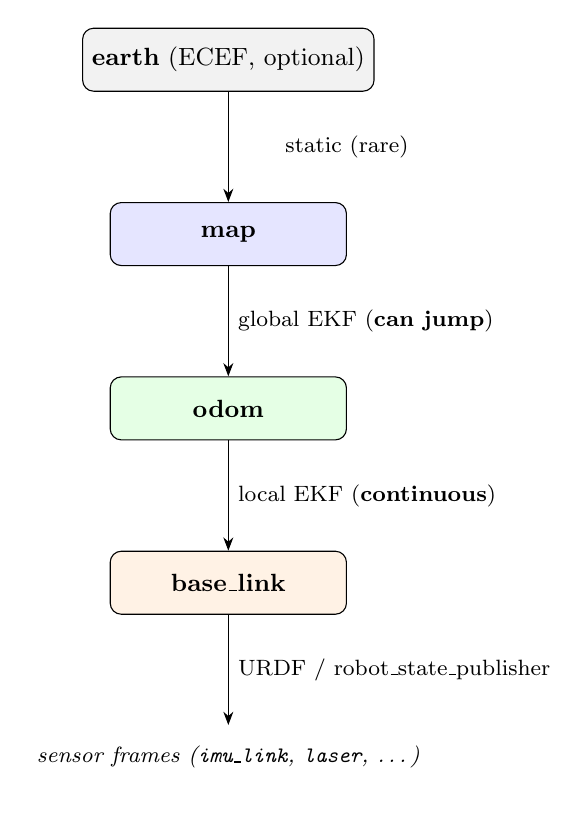
\begin{tikzpicture}[node distance=1.4cm, every node/.style={draw, rounded corners, minimum width=3.0cm, minimum height=0.8cm, font=\small}, ->,>=Stealth]
\node (earth) [fill=gray!10] {\textbf{earth} (ECEF, optional)};
\node (map) [below=of earth, fill=blue!10] {\textbf{map}};
\node (odom) [below=of map, fill=green!10] {\textbf{odom}};
\node (base) [below=of odom, fill=orange!10] {\textbf{base\_link}};
\node (sens) [below=of base, draw=none, font=\footnotesize\itshape] {sensor frames (\texttt{imu\_link}, \texttt{laser}, \ldots)};
\draw (earth) -- node[right, draw=none, font=\footnotesize] {static (rare)} (map);
\draw (map) -- node[right, draw=none, font=\footnotesize] {global EKF (\textbf{can jump})} (odom);
\draw (odom) -- node[right, draw=none, font=\footnotesize] {local EKF (\textbf{continuous})} (base);
\draw (base) -- node[right, draw=none, font=\footnotesize] {URDF / robot\_state\_publisher} (sens);
\end{tikzpicture}
\end{center}

\textbf{Frame definitions:}
\begin{itemize}
\item \texttt{earth}: ECEF (Earth-Centered, Earth-Fixed). Used for multi-robot or surveying. Usually omitted.
\item \texttt{map}: world-fixed reference. Globally consistent. Origin chosen at startup or pre-defined. ENU axes (X-East, Y-North, Z-Up) by convention.
\item \texttt{odom}: world-fixed reference for the robot. Drifts over time but \textbf{continuous}. Origin at robot's startup pose typically.
\item \texttt{base\_link}: rigidly attached to robot body. Convention: X forward, Y left, Z up.
\item Sensor frames: rigidly attached to body via static transforms from URDF.
\end{itemize}

\subsection{Why Two Frames? Why Two EKFs?}

ROS Navigation Stack imposes a hard constraint:

\begin{warnbox}{Navigation Constraint}
The transform \texttt{odom} $\to$ \texttt{base\_link} must be \textbf{continuous} and \textbf{monotonic}. No jumps. Ever.
\end{warnbox}

Local planner integrates pose forward to compute trajectories and velocity commands. Discontinuity in \texttt{base\_link} pose would make controller believe robot teleported --- catastrophic control commands emitted.

But absolute references like GPS \emph{do} produce position corrections, sometimes large. Need somewhere to absorb these jumps. Solution: \textbf{decouple the transform chain}.

\begin{center}
\begin{tabular}{lll}
\toprule
\textbf{Transform} & \textbf{Continuous?} & \textbf{Purpose}\\
\midrule
\texttt{odom} $\to$ \texttt{base\_link} & Yes (smooth) & Local planning, control \\
\texttt{map} $\to$ \texttt{odom} & No (can jump) & Global path planning \\
\bottomrule
\end{tabular}
\end{center}

When GPS provides correction, only \texttt{map} $\to$ \texttt{odom} jumps; \texttt{odom} $\to$ \texttt{base\_link} unaffected. Robot pose in map frame = composition of both transforms, absorbs correction cleanly:
\[
T_{\text{map}}^{\text{base}} = T_{\text{map}}^{\text{odom}} \cdot T_{\text{odom}}^{\text{base}}
\]

When GPS jumps, $T_{\text{map}}^{\text{odom}}$ adjusts to compensate for accumulated $T_{\text{odom}}^{\text{base}}$ drift, leaving $T_{\text{map}}^{\text{base}}$ globally accurate.

% ========================================================================
\section{robot\_localization Architecture}
% ========================================================================

\subsection{Node Topology}

\begin{center}
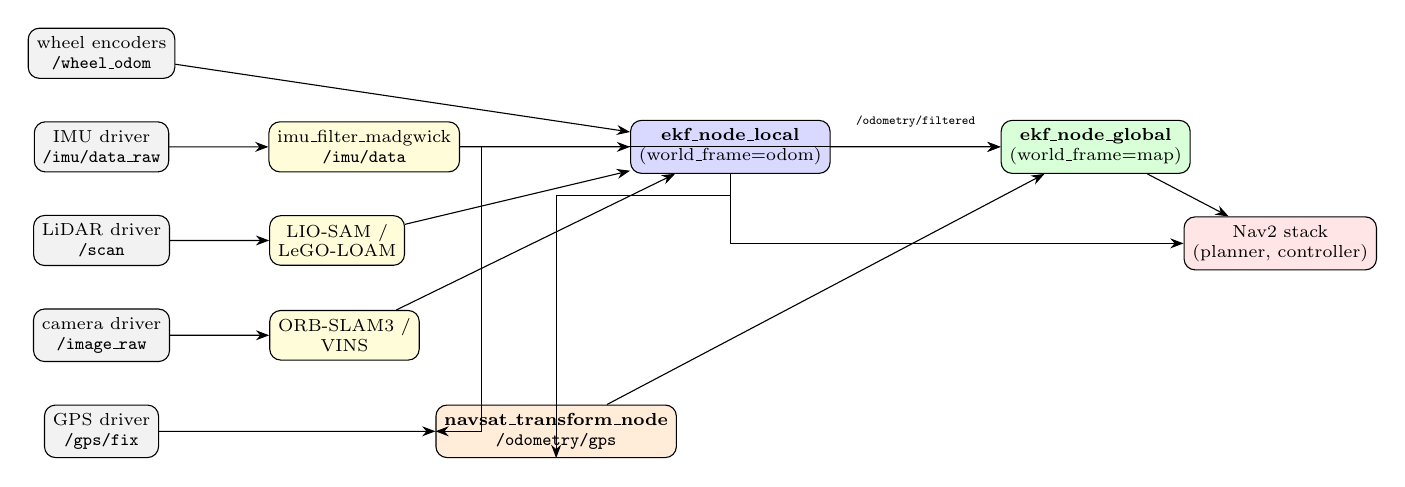
\begin{tikzpicture}[
  node distance=0.6cm and 1.4cm,
  every node/.style={draw, rounded corners, font=\scriptsize, minimum height=0.7cm, align=center},
  ->,>=Stealth, scale=0.9, transform shape
]
% Sensor sources
\node[fill=gray!10] (wheel) {wheel encoders\\\texttt{/wheel\_odom}};
\node[fill=gray!10, below=of wheel] (imu) {IMU driver\\\texttt{/imu/data\_raw}};
\node[fill=gray!10, below=of imu] (lidar) {LiDAR driver\\\texttt{/scan}};
\node[fill=gray!10, below=of lidar] (cam) {camera driver\\\texttt{/image\_raw}};
\node[fill=gray!10, below=of cam] (gps) {GPS driver\\\texttt{/gps/fix}};

% Pre-processing
\node[fill=yellow!15, right=of imu] (madgwick) {imu\_filter\_madgwick\\\texttt{/imu/data}};
\node[fill=yellow!15, right=of lidar] (lidarodom) {LIO-SAM /\\LeGO-LOAM};
\node[fill=yellow!15, right=of cam] (vo) {ORB-SLAM3 /\\VINS};

% Local EKF
\node[fill=blue!15, right=of madgwick, xshift=1.0cm] (lekf) {\textbf{ekf\_node\_local}\\(world\_frame=odom)};

% navsat_transform
\node[fill=orange!15, right=of gps, xshift=2.5cm] (nav) {\textbf{navsat\_transform\_node}\\\texttt{/odometry/gps}};

% Global EKF
\node[fill=green!15, right=of lekf, xshift=1.0cm] (gekf) {\textbf{ekf\_node\_global}\\(world\_frame=map)};

% Outputs
\node[fill=red!10, below right=of gekf, xshift=-1.5cm] (nav2) {Nav2 stack\\(planner, controller)};

% Connections
\draw (wheel) -- (lekf);
\draw (imu) -- (madgwick);
\draw (madgwick) -- (lekf);
\draw (madgwick.east) -- ++(0.3,0) |- (gekf);
\draw (madgwick.east) -- ++(0.3,0) |- (nav);
\draw (lidar) -- (lidarodom);
\draw (lidarodom) -- (lekf);
\draw (cam) -- (vo);
\draw (vo) -- (lekf);
\draw (gps) -- (nav);
\draw (lekf) -- node[font=\tiny, draw=none, above]{\texttt{/odometry/filtered}} (gekf);
\draw (lekf.south) -- ++(0,-0.3) -| (nav.south);
\draw (nav) -- (gekf);
\draw (gekf) -- (nav2);
\draw (lekf) |- (nav2);
\end{tikzpicture}
\end{center}

\subsection{Node-by-Node Walkthrough}

\subsubsection{ekf\_node\_local (Local EKF)}

\textbf{Package:} \texttt{robot\_localization}\\
\textbf{Executable:} \texttt{ekf\_node}\\
\textbf{Role:} Fuse continuous-only sensors into smooth local pose estimate.

\textbf{Subscribes to:}
\begin{itemize}
\item \texttt{/wheel\_odom} (\texttt{nav\_msgs/Odometry}) --- wheel encoder velocities
\item \texttt{/imu/data} (\texttt{sensor\_msgs/Imu}) --- filtered IMU
\item \texttt{/lidar\_odom} (\texttt{nav\_msgs/Odometry}) --- LiDAR odometry (optional)
\item \texttt{/visual\_odom} (\texttt{nav\_msgs/Odometry}) --- visual odometry (optional)
\end{itemize}

\textbf{Publishes:}
\begin{itemize}
\item \texttt{/odometry/filtered} (\texttt{nav\_msgs/Odometry}) --- fused state, in \texttt{odom} frame
\item TF: \texttt{odom} $\to$ \texttt{base\_link} (continuous)
\item \texttt{/diagnostics} (\texttt{diagnostic\_msgs/DiagnosticArray})
\end{itemize}

\textbf{Configuration parameters (key):}
\begin{lstlisting}[language=bash]
ekf_node_local:
  ros__parameters:
    frequency: 50.0                       # filter publish rate Hz
    sensor_timeout: 0.1                   # s before marking sensor offline
    two_d_mode: true                      # planar robot (zero z, roll, pitch)
    publish_tf: true
    publish_acceleration: false

    map_frame:       map
    odom_frame:      odom
    base_link_frame: base_link
    world_frame:     odom                 # KEY: local EKF in odom frame

    # Sensor 0: wheel odometry (use velocities only)
    odom0: /wheel_odom
    odom0_config: [false, false, false,   # x, y, z position
                   false, false, false,   # roll, pitch, yaw
                   true,  false, false,   # vx, vy, vz
                   false, false, true,    # vroll, vpitch, vyaw
                   false, false, false]   # ax, ay, az
    odom0_differential: false
    odom0_relative: false
    odom0_queue_size: 10

    # Sensor 1: IMU (orientation + angular velocities)
    imu0: /imu/data
    imu0_config: [false, false, false,
                  true,  true,  false,    # roll, pitch (no yaw if no mag)
                  false, false, false,
                  true,  true,  true,     # all angular velocities
                  true,  true,  false]    # planar accels
    imu0_differential: false
    imu0_remove_gravitational_acceleration: true

    # Process noise (R_t in Thrun notation)
    process_noise_covariance: [0.05, 0,    0,    ...,   # x
                               0,    0.05, 0,    ...,   # y
                               ...]
    initial_estimate_covariance: [1e-9, 0, 0, ...]
\end{lstlisting}

\textbf{Internal state vector (15D):}
\[
\mu_t = [x,\, y,\, z,\, \phi,\, \theta,\, \psi,\, \dot{x},\, \dot{y},\, \dot{z},\, \dot{\phi},\, \dot{\theta},\, \dot{\psi},\, \ddot{x},\, \ddot{y},\, \ddot{z}]^\top
\]

In \texttt{two\_d\_mode: true}, components $z, \phi, \theta, \dot{z}, \dot{\phi}, \dot{\theta}, \ddot{z}$ are clamped to zero.

\subsubsection{ekf\_node\_global (Global EKF)}

\textbf{Same executable, different config.} Sets \texttt{world\_frame: map}. The role differs sharply between the canonical \texttt{robot\_localization} tutorial pattern and the architecture used in this project.

\paragraph{Canonical pattern (Tom Moore reference example).}
Both EKFs subscribe to the \emph{same raw sensors} (wheel odom, IMU). Global EKF additionally subscribes to \texttt{/odometry/gps} from \texttt{navsat\_transform\_node}. GPS provides absolute position correction; map frame stays globally anchored.

\paragraph{Project pattern (Husarion Lynx, this codebase).}
Global EKF \textbf{deliberately excludes GPS}. Both EKFs receive identical sensor inputs (wheel + VO + LiDAR + IMU), differing only in \texttt{world\_frame}. GPS still flows through \texttt{navsat\_transform\_node} and is published on \texttt{/odometry/gps} for analysis, but it is \emph{not} listed in EKF~\#2's sensor inputs. The reason for this departure is detailed in the next subsection (covariance cross-term leak); briefly, single-antenna GPS noise injected into a filter without a strong yaw observation produces a $\sim$3.56°/s yaw drift in the map frame.

\textbf{Subscribes to (this project):}
\begin{itemize}
\item \texttt{/diff\_drive\_controller/odom} --- raw wheel odometry (twist only)
\item \texttt{/imu/data} --- IMU (orientation, angular velocity, acceleration)
\item \texttt{/odometry/visual} --- RTAB-Map visual odometry
\item \texttt{/odometry/lidar} --- ICP LiDAR odometry
\item (NOT \texttt{/odometry/gps})
\end{itemize}

\textbf{Publishes:}
\begin{itemize}
\item \texttt{/odometry/filtered\_map} --- fused state in \texttt{map} frame
\item TF: \texttt{map} $\to$ \texttt{odom} (\textbf{near-identity} in this project; can jump in canonical pattern)
\end{itemize}

\textbf{Config delta (canonical pattern):}
\begin{lstlisting}[language=bash]
ekf_node_global:
  ros__parameters:
    world_frame: map

    odom0: /wheel/odometry                # SAME raw sensor as local EKF
    odom0_config: [false, false, false,
                   false, false, false,
                   true,  false, false,
                   false, false, true,
                   false, false, false]

    imu0: /imu/data                       # SAME raw sensor as local EKF

    odom1: /odometry/gps                  # only canonical: enable GPS here
    odom1_config: [true, true, false,
                   false, false, false,
                   false, false, false,
                   false, false, false,
                   false, false, false]
\end{lstlisting}

\textbf{Config delta (project, GPS excluded):}
\begin{lstlisting}[language=bash]
ekf_node_global:
  ros__parameters:
    world_frame: map

    odom0: /diff_drive_controller/odom    # raw wheel
    odom1: /odometry/visual               # raw VO
    odom2: /odometry/lidar                # raw LO
    imu0:  /imu/data                      # raw IMU
    # GPS is INTENTIONALLY OMITTED - see Section on covariance leak
\end{lstlisting}

\begin{warnbox}{Common Misconception}
A frequent misconfiguration is feeding \texttt{/odometry/filtered} (local EKF output) into the global EKF as a sensor input. This creates a chain where the global filter consumes the local filter's already-fused estimate. Per Tom Moore's reference example (\texttt{cra-ros-pkg/robot\_localization/params/dual\_ekf\_navsat\_example.yaml}), both EKFs must subscribe to the \emph{same raw sensors independently}, in parallel. Chaining produces:
\begin{itemize}
\item Double-counting of measurement information
\item Covariance accounting that diverges from optimal
\item Feedback loop with \texttt{navsat\_transform\_node} (which already reads \texttt{/odometry/filtered})
\end{itemize}
\end{warnbox}

\subsubsection{navsat\_transform\_node}

\textbf{Package:} \texttt{robot\_localization}\\
\textbf{Executable:} \texttt{navsat\_transform\_node}\\
\textbf{Role:} Convert \texttt{NavSatFix} (lat, lon, alt) into \texttt{Odometry} in \texttt{map} frame.

\textbf{Subscribes to:}
\begin{itemize}
\item \texttt{/gps/fix} (\texttt{sensor\_msgs/NavSatFix}) --- raw GPS
\item \texttt{/imu/data} (\texttt{sensor\_msgs/Imu}) --- for initial heading
\item \texttt{/odometry/filtered} --- fused robot pose for transform anchoring
\end{itemize}

\textbf{Publishes:}
\begin{itemize}
\item \texttt{/odometry/gps} (\texttt{nav\_msgs/Odometry}) --- GPS measurement in map frame, ready for global EKF
\item \texttt{/gps/filtered} (\texttt{sensor\_msgs/NavSatFix}) --- GPS in lat/lon corresponding to filtered state
\end{itemize}

\textbf{Internal pipeline:}

\begin{enumerate}
\item \textbf{LL2UTM conversion}: latitude/longitude $\to$ UTM (Universal Transverse Mercator) coordinates. UTM is a metric, locally Cartesian projection. The Earth surface is divided into 60 zones of $6^\circ$ longitude. Inside each zone, conversion is essentially:
\begin{align*}
N &= k_0\, A_0 + (\text{series in } \phi, \lambda) \\
E &= k_0\, [\text{series in } \phi, \lambda] + 500{,}000
\end{align*}
where $k_0 = 0.9996$ is the central meridian scale factor. Output: $(E_{\text{UTM}}, N_{\text{UTM}})$ in metres.

\item \textbf{Datum establishment}: on first GPS fix (or from \texttt{datum} parameter), record the initial UTM coordinates as origin:
\[
(E_0, N_0) = (E_{\text{UTM}}^{(0)}, N_{\text{UTM}}^{(0)})
\]

\item \textbf{Local Cartesian offset}:
\[
(x_{\text{local}}, y_{\text{local}}) = (E_{\text{UTM}} - E_0,\; N_{\text{UTM}} - N_0)
\]

\item \textbf{Heading rotation}: map frame's $+x$ axis may not coincide with UTM East. Rotate by initial yaw $\psi_0$:
\[
\begin{bmatrix}x_{\text{map}} \\ y_{\text{map}}\end{bmatrix} = \begin{bmatrix}\cos\psi_0 & \sin\psi_0 \\ -\sin\psi_0 & \cos\psi_0\end{bmatrix}\begin{bmatrix}x_{\text{local}} \\ y_{\text{local}}\end{bmatrix}
\]
$\psi_0$ obtained from magnetometer heading at startup, or set explicitly via \texttt{yaw\_offset} param.

\item \textbf{Publish}: $(x_{\text{map}}, y_{\text{map}})$ as \texttt{Odometry} message with covariance computed from GPS fix's reported HDOP/VDOP.
\end{enumerate}

\textbf{Configuration:}
\begin{lstlisting}[language=bash]
navsat_transform_node:
  ros__parameters:
    frequency: 30.0
    delay: 3.0                            # wait for sensor fixes to stabilise
    magnetic_declination_radians: 0.0     # local magnetic declination (look up!)
    yaw_offset: 0.0                       # IMU 0 yaw vs map +X axis offset
    zero_altitude: true                   # ignore altitude (planar robot)
    publish_filtered_gps: true
    use_odometry_yaw: false               # use IMU yaw, not odom yaw, for datum
    wait_for_datum: false                 # auto-set datum on first fix
    # Or explicit datum:
    # datum: [55.944904, -3.186693, 0.0]  # lat, lon, yaw
\end{lstlisting}

\textbf{Magnetic declination}: the angle between true north and magnetic north at your location. Varies geographically ($-20^\circ$ to $+20^\circ$ globally). Look up via NOAA's geomagnetic calculator.

\subsubsection{imu\_filter\_madgwick (Pre-Filter)}

\textbf{Package:} \texttt{imu\_filter\_madgwick}\\
\textbf{Role:} Convert raw accelerometer + gyroscope (+ magnetometer) into a stable orientation estimate. Subscribes to \texttt{/imu/data\_raw}, publishes \texttt{/imu/data} with orientation field populated.

Madgwick filter is a complementary-filter family algorithm: gyro integration with gradient-descent correction toward gravity (for roll/pitch) and magnetic field (for yaw). Cheaper than EKF, robust, used widely.

This pre-filter exists because most cheap IMUs publish only raw rates and accelerations --- no orientation. The downstream EKF expects orientation in the IMU message.

\subsubsection{LiDAR Odometry Node (e.g., LIO-SAM)}

External node (not part of \texttt{robot\_localization}). Performs scan-matching + IMU preintegration + factor-graph optimisation. Publishes \texttt{nav\_msgs/Odometry} with 6-DOF pose and twist + covariance.

\subsection{Topic and TF Flow Summary}

\begin{center}
\footnotesize
\begin{tabular}{lll}
\toprule
\textbf{Topic / TF} & \textbf{Source} & \textbf{Sink}\\
\midrule
\texttt{/diff\_drive\_controller/odom} & wheel driver & \textbf{both} EKFs (parallel) \\
\texttt{/imu/data\_raw} & IMU driver & madgwick filter \\
\texttt{/imu/data} & madgwick & \textbf{both} EKFs (parallel), navsat \\
\texttt{/gps/fix} & GPS driver & navsat (canonical also $\to$ global EKF) \\
\texttt{/scan} or \texttt{/points} & LiDAR driver & LiDAR odom node \\
\texttt{/odometry/lidar} & LiDAR odom & \textbf{both} EKFs (parallel) \\
\texttt{/odometry/visual} & VO node & \textbf{both} EKFs (parallel) \\
\texttt{/odometry/filtered} & local EKF & navsat (datum bootstrap), Nav2 \\
\texttt{/odometry/gps} & navsat & global EKF (canonical) / analysis only (project) \\
\texttt{/odometry/filtered\_map} & global EKF & Nav2 (planner) \\
TF \texttt{odom} $\to$ \texttt{base\_link} & local EKF & TF tree (continuous) \\
TF \texttt{map} $\to$ \texttt{odom} & global EKF & TF tree (jumps in canonical, $\approx I$ in project) \\
TF \texttt{base\_link} $\to$ sensor & URDF / static & TF tree \\
\bottomrule
\end{tabular}
\end{center}

\subsection{Why Each Sensor Goes Where}

\textbf{Canonical pattern:}
\begin{itemize}
\item \textbf{Wheel odom $\to$ both EKFs (parallel)}: high-rate smooth velocities. Same raw msg fed to both.
\item \textbf{IMU $\to$ both EKFs (parallel)}: high-rate orientation + angular velocity. Same raw msg fed to both.
\item \textbf{LiDAR/Visual odom $\to$ both EKFs}: continuous pose deltas, both filters benefit.
\item \textbf{GPS $\to$ global EKF only}: GPS jumps would break local continuity. Goes only to global via navsat.
\end{itemize}

\textbf{Project pattern (this codebase):}
\begin{itemize}
\item \textbf{Wheel, IMU, VO, LiDAR $\to$ both EKFs (parallel)}: identical sensor consensus across both filters.
\item \textbf{GPS $\to$ navsat\_transform only, NOT into either EKF}: GPS published on \texttt{/odometry/gps} but excluded from both EKF input lists. Available for analysis, ignored for fusion.
\end{itemize}

The project pattern produces \texttt{map} $\to$ \texttt{odom} $\approx$ identity transform (typically $\pm 0.1$ m translation, $\pm 1°$ rotation over a 2-minute run) because both filters process identical inputs and converge to nearly identical state estimates.

\subsection{The Covariance Cross-Term Leak (Why GPS is Excluded in this Project)}
\label{sec:covariance-leak}

This is the core engineering reason behind the project's deliberate departure from canonical dual-EKF + NavSat. The phenomenon is subtle but has measurable consequences (3.56°/s map frame yaw drift in this project's earlier configuration with GPS enabled).

\subsubsection{The Mechanism}

The EKF state covariance $\Sigma$ is a dense $15 \times 15$ matrix --- not diagonal. Off-diagonal entries $\Sigma_{x,\psi}$ and $\Sigma_{y,\psi}$ encode statistical correlation: ``if I learn something about $x$, what does it tell me about yaw $\psi$?''

These cross-terms become non-zero whenever the robot moves with $\omega \neq 0$ because the motion-model Jacobian $G_t$ has a non-zero $\partial g_x / \partial \psi$ entry:
\[
G_t = \begin{bmatrix} 1 & 0 & -v\sin(\mu_\theta)\Delta t \\ 0 & 1 & v\cos(\mu_\theta)\Delta t \\ 0 & 0 & 1 \end{bmatrix}
\]

Predicted covariance $\bar{\Sigma}_t = G_t\,\Sigma_{t-1}\,G_t^\top + R_t$ inherits cross-terms from this Jacobian. After any curved motion, $\Sigma_{x,\psi}, \Sigma_{y,\psi} \neq 0$.

\subsubsection{The Leak Path}

When a GPS measurement arrives, $H_{\text{GPS}}$ selects only $[x, y]$. But the Kalman gain $K_t = \bar{\Sigma}_t H_t^\top S_t^{-1}$ has a row for \emph{every} state component, including yaw. The yaw update entry:
\[
K_{\psi, x} = \frac{\Sigma_{\psi,x}}{\Sigma_{xx} + Q_{\text{GPS}}}
\]

GPS noise $\sigma_{\text{GPS}} \approx 0.5$ m produces innovation $\nu_x \neq 0$ on every cycle. Yaw correction:
\[
\Delta\psi = K_{\psi,x}\,\nu_x + K_{\psi,y}\,\nu_y
\]

\textbf{GPS never observed yaw, but yaw moved.} Each fix injects a small angular correction.

\subsubsection{Compounding}

The Joseph form covariance update reduces but does not eliminate the cross-term:
\[
\Sigma_{\psi,x}^{\text{new}} = \Sigma_{\psi,x} - K_{\psi,x}\,\Sigma_{xx}
\]

Then the next predict step regrows it via $G_t$. Subsequent VO or LiDAR updates --- which observe both position and yaw --- amplify the leak by simultaneously correcting position (matching the GPS-shifted estimate) and re-using the now-shaped covariance.

Result: yaw drift compounds at $\approx 3.56°/$s in the configured system.

\subsubsection{Numerical Walk-Through (Project Values)}

State after some driving (illustrative):
\[
\Sigma_{xx} = 0.30 \text{ m}^2, \quad \Sigma_{\psi\psi} = 0.02 \text{ rad}^2, \quad \Sigma_{x,\psi} = 0.04
\]

GPS innovation $\nu_x = 0.5$ m (typical noise spike), $Q_{\text{GPS}} = 0.26$ m$^2$:
\[
K_{\psi,x} = \frac{0.04}{0.30 + 0.26} \approx 0.071
\]
\[
\Delta\psi = 0.071 \cdot 0.5 \approx 0.036 \text{ rad} \approx 2°
\]

Single GPS fix moved yaw by 2° via cross-term coupling. At 10 Hz GPS, even with partial randomness in direction, sustained walk emerges.

\subsubsection{Why the Canonical Tutorial Doesn't Suffer This}

Tom Moore's canonical configuration assumes a strong absolute yaw observation, typically from:
\begin{itemize}
\item Dual-antenna RTK GPS providing measured heading
\item Reliable magnetometer with proper hard/soft-iron calibration
\item Visual landmarks with known orientation (rare)
\end{itemize}

Under those conditions, an absolute yaw measurement is provided each cycle. Its measurement-noise covariance $Q_\psi$ is small. The Kalman gain heavily weights this direct yaw observation, dominating the indirect leak from GPS cross-terms. Yaw stays bounded.

In this project, the simulated IMU has \emph{no magnetometer}; the system has \emph{no dual-antenna RTK}. Yaw is integrated from gyro only --- no absolute observation. Nothing fights the leak.

\subsubsection{The Sensor Consensus Solution}

By feeding both EKFs identical sensor sets --- and \emph{omitting GPS from EKF \#2} --- the project enforces:
\begin{equation}
\mu_t^{(\text{global})} \approx \mu_t^{(\text{local})} \implies T_{\text{map}}^{\text{odom}} \approx I
\end{equation}

The map $\to$ odom transform stays near-identity. No GPS-driven cross-term leakage. Map frame angularly stable.

\textbf{Trade-off:} The map frame is no longer GPS-anchored to absolute world coordinates. The robot's map-frame pose drifts with wheel/IMU drift over arbitrary distances. For indoor/short-range outdoor missions where global georeferencing is not required, this is acceptable.

\subsubsection{Alternatives if Global Anchoring is Required}

If you need both global anchoring \emph{and} no leak:
\begin{enumerate}
\item \textbf{Add a strong yaw observation}: dual-antenna RTK, calibrated magnetometer, or sun sensor.
\item \textbf{Diagonalise $\Sigma$ after GPS update}: zero out $\Sigma_{x,\psi}, \Sigma_{y,\psi}$ post-correction. Hacky but eliminates leak. Requires custom EKF code (not available in stock \texttt{robot\_localization}).
\item \textbf{Loosely-coupled GPS in a separate filter}: run a third filter that consumes only EKF~\#2 output and GPS, then publish a \texttt{utm}~$\to$~\texttt{map} transform without polluting EKF~\#2's state.
\item \textbf{Periodic re-anchoring}: when GPS confidence is high (e.g., RTK fix), do a one-shot pose reset of EKF~\#2 instead of continuous fusion.
\end{enumerate}

\begin{insightbox}{Empirical Evidence in this Project}
Earlier configuration (GPS in EKF~\#2): map frame yaw drifted at 3.56°/s sustained, accumulating to over 200° in 2 minutes --- catastrophic for navigation.

Current configuration (GPS removed from EKF~\#2): map~$\to$~odom transform stays within $\pm 0.1$ m and $\pm 1°$ over a 2-minute run.

The diagnosis trace:
\begin{enumerate}
\item Disable GPS in EKF~\#2 $\to$ drift disappears.
\item Re-enable GPS $\to$ drift returns.
\item Disable VO and LiDAR (only wheel + IMU + GPS) $\to$ drift much reduced because no second update path amplifies the cross-term.
\end{enumerate}
The cross-term leak is the cause; sensor consensus is the cure.
\end{insightbox}

% ========================================================================
\section{The EKF Execution Loop}
% ========================================================================

\subsection{Local EKF Pseudocode}

\begin{lstlisting}[language=Python]
# Initialization
mu = np.zeros(15)                  # state mean
Sigma = initial_covariance()       # state covariance
last_t = ros_time_now()

# Main loop @ frequency parameter (e.g. 50 Hz)
while node_ok():
    now = ros_time_now()
    dt = now - last_t
    last_t = now

    # === PREDICT ===
    # Apply nonlinear motion model g
    mu_bar = g(mu, dt)
    G = jacobian_g(mu, dt)
    Sigma_bar = G @ Sigma @ G.T + R * dt   # process noise R scaled by dt

    # === CORRECT (per pending measurement) ===
    for sensor_msg in get_pending_measurements_in_time_order():
        z = sensor_msg.measurement
        Q = sensor_msg.covariance
        h = sensor_msg.h_function
        H = sensor_msg.H_jacobian(mu_bar)

        # Innovation
        innov = z - h(mu_bar)
        innov = wrap_angles(innov)         # critical for orientation

        # Mahalanobis gating
        S = H @ Sigma_bar @ H.T + Q
        d2 = innov.T @ np.linalg.inv(S) @ innov
        if d2 > CHI2_99[len(z)]:
            continue                       # outlier

        # Kalman gain
        K = Sigma_bar @ H.T @ np.linalg.inv(S)

        # Update
        mu_bar = mu_bar + K @ innov
        I_KH = np.eye(15) - K @ H
        Sigma_bar = I_KH @ Sigma_bar @ I_KH.T + K @ Q @ K.T   # Joseph

    mu, Sigma = mu_bar, Sigma_bar

    # === PUBLISH ===
    publish_tf("odom", "base_link", mu[:3], quat_from_euler(mu[3:6]))
    publish_odometry("/odometry/filtered", mu, Sigma)
\end{lstlisting}

\subsection{Multi-Sensor Update Order}

When multiple measurements arrive in same cycle, process sequentially in time order. \texttt{robot\_localization} buffers measurements by timestamp, processes chronologically. Allows \emph{retroactive correction}: if delayed measurement arrives, filter rolled back to its timestamp, measurement applied, filter re-stepped forward. Implementation: ring buffer of past states.

\subsection{Prediction-Only Periods}

Between GPS fixes (e.g., 1 Hz GPS, 50 Hz filter):
\begin{verbatim}
t=0.00: GPS update    -> Sigma shrinks
t=0.02: Predict       -> Sigma grows slightly
...
t=0.98: Predict       -> Sigma grown considerably
t=1.00: GPS update    -> Sigma shrinks
\end{verbatim}
``Breath'' of filter. After 1 s of dead reckoning with $\sigma_{\dot{x}} = 0.1$ m/s, position uncertainty grows by $\approx 0.1$ m.

% ========================================================================
\section{Wheel Odometry: Theory and Practice}
% ========================================================================

\subsection{Hardware: Quadrature Encoders}

A quadrature encoder is two photodetectors (or magnetic Hall sensors) reading a slotted disc on the wheel axle. Two channels A and B physically offset by $90^\circ$ of the slot pattern, producing two square waves in quadrature:

\begin{verbatim}
Channel A: |##__|##__|##__|##__|
Channel B: ##|__|##__|##__|##__|
\end{verbatim}

Forward rotation: A leads B. Reverse: B leads A. Counting transitions on both channels gives $4N$ counts per revolution where $N$ is slot count --- ``$\times 4$ decoding''. Typical robotics encoders: 1024--4096 CPR after $\times 4$. With gearing, output-shaft resolution much higher.

\subsection{Differential-Drive Kinematics}

Define:
\begin{itemize}
\item $r$: wheel radius
\item $b$: wheel baseline (track width, distance between left/right wheels)
\item $\Delta n_L, \Delta n_R$: encoder counts on left/right wheels during $\Delta t$
\item $N_{\text{CPR}}$: counts per revolution (after $\times 4$)
\end{itemize}

Linear wheel velocities (m/s):
\[
v_L = \frac{2\pi r\, \Delta n_L}{N_{\text{CPR}}\, \Delta t}, \qquad v_R = \frac{2\pi r\, \Delta n_R}{N_{\text{CPR}}\, \Delta t}
\]

Robot body-frame velocities:
\begin{equation}
\boxed{\;v = \frac{v_R + v_L}{2}, \qquad \omega = \frac{v_R - v_L}{b}\;}
\end{equation}

These two scalars $(v, \omega)$ are the entire output of the kinematic model.

\subsection{Pose Integration}

\textbf{Euler integration} (first-order, accumulates more error):
\[
x_{t+1} = x_t + v\cos(\theta_t)\Delta t, \quad y_{t+1} = y_t + v\sin(\theta_t)\Delta t, \quad \theta_{t+1} = \theta_t + \omega\Delta t
\]

\textbf{Runge-Kutta 2nd-order (midpoint)} --- evaluate orientation at midpoint:
\[
x_{t+1} = x_t + v\cos\!\left(\theta_t + \tfrac{\omega\Delta t}{2}\right)\Delta t, \quad y_{t+1} = y_t + v\sin\!\left(\theta_t + \tfrac{\omega\Delta t}{2}\right)\Delta t
\]

\textbf{Exact integration} for constant $(v, \omega)$ over interval (when $\omega \neq 0$, motion on circular arc):
\[
\Delta x = \frac{v}{\omega}[\sin(\theta_t + \omega\Delta t) - \sin(\theta_t)]
\]
\[
\Delta y = -\frac{v}{\omega}[\cos(\theta_t + \omega\Delta t) - \cos(\theta_t)]
\]
\[
\Delta \theta = \omega \Delta t
\]
For $\omega \to 0$: straight-line case recovered.

\subsection{What the EKF Receives}

Crucial choice: feed the EKF \emph{integrated pose} or \emph{velocity (twist)}?

\textbf{Best practice: feed twist, not pose.} EKF performs own integration, fusing wheel + IMU. Feeding pre-integrated pose causes double integration of encoder noise. Feed instantaneous velocities, let filter integrate with all sensors weighted properly.

\begin{lstlisting}[language=bash]
odom0: /wheel_odom
odom0_config: [false, false, false,    # don't use position
               false, false, false,    # don't use orientation
               true,  false, false,    # USE twist v_x
               false, false, true,     # USE twist omega_z
               false, false, false]    # don't use accel
\end{lstlisting}

\subsection{Error Sources}

\textbf{1. Wheel slip.} Actual ground travel differs from encoder count:
\[
v_{\text{true}} = v_{\text{measured}} \cdot (1 - s), \quad s \in [0, 1]
\]
$s$ spikes near 1 on ice or sharp acceleration. EKF cannot distinguish slip from real motion --- relies on IMU/GPS to catch.

\textbf{2. Wheel radius miscalibration.} Assumed $\hat{r}$ vs true $r$:
\[
\frac{e_v}{v} = \frac{r - \hat{r}}{\hat{r}}
\]
Constant scale error. Position drift grows linearly with distance. Tire wear and pressure variation drift this over time.

\textbf{3. Baseline miscalibration.} Assumed $\hat{b}$ vs true $b$:
\[
\frac{e_\omega}{\omega} = \frac{b - \hat{b}}{\hat{b}}
\]
Heading error per turn. Manifests as systematic curvature: robot commanded straight spirals slowly.

\textbf{4. Encoder quantisation.}
\[
\sigma_{v,\text{quant}} \approx \frac{2\pi r}{N_{\text{CPR}}\, \Delta t \sqrt{12}}
\]

\textbf{5. Random walk drift.} On flat terrain with i.i.d.\ noise, position uncertainty grows as $\sqrt{d}$ where $d$ is distance travelled. Systematic bias makes error grow linearly.

\subsection{Noise Model}

\[
Q_{\text{wheel}} = \begin{bmatrix}\sigma_{v_x}^2 & 0 \\ 0 & \sigma_{\omega_z}^2\end{bmatrix}
\]
Typical small mobile robot:
\begin{itemize}
\item $\sigma_{v_x} \approx 0.05$--$0.1$ m/s
\item $\sigma_{\omega_z} \approx 0.02$--$0.05$ rad/s
\end{itemize}
Tune empirically: drive known trajectory, compare integrated pose to ground truth, increase covariance until residual consistent with gating.

% ========================================================================
\section{IMU: Theory and Practice}
% ========================================================================

\subsection{MEMS Inertial Sensors}

Modern IMUs are MEMS (Micro-Electro-Mechanical Systems) devices etched in silicon at micron scale.

\subsubsection{Accelerometer}

Proof mass $m$ suspended by silicon spring beams between fixed electrodes. Linear acceleration along sensitive axis displaces mass, changing capacitance:
\[
C = \frac{\varepsilon A}{d}
\]
$d$ is gap. Differential capacitive sensing measures gap change to nanometre precision. Deflection proportional to specific force along axis.

\textbf{Critical fact:} accelerometer measures \emph{specific force}, not pure acceleration. Output:
\begin{equation}
\boxed{\;\tilde{a}^b = a^b_{\text{true}} - R^b_w\, g + b_a + n_a\;}
\end{equation}
where $R^b_w$ rotates world-frame gravity $g = [0,0,-9.81]^\top$ into body frame. Free-falling accelerometer reads zero. Stationary accelerometer reads $-g$ rotated into body frame --- pointing ``up''.

\subsubsection{Gyroscope (Coriolis MEMS)}

Vibrating mass driven at resonant frequency along drive axis. Package rotation induces Coriolis force, deflecting mass along sense axis:
\[
F_{\text{Coriolis}} = -2m(\Omega \times v_{\text{drive}})
\]
Deflection amplitude proportional to angular velocity $\Omega$. Output:
\begin{equation}
\boxed{\;\tilde{\omega}^b = \omega^b_{\text{true}} + b_g + n_g\;}
\end{equation}

\subsubsection{Magnetometer (9-DOF IMUs)}

Hall-effect or magnetoresistive sensor measures local magnetic field. Ideally points to magnetic north, gives absolute yaw. Practice: corrupted by hard-iron (permanent magnets), soft-iron (ferromagnetic distortion), environmental anomalies (steel structures, motors). Indoor robots often disable magnetometer.

\subsection{Allan Variance Noise Model}

Allan variance plot is canonical IMU noise characterisation. Plot $\sigma_{\text{Allan}}(\tau)$ vs averaging time $\tau$ on log-log axes:

\begin{center}
\begin{tikzpicture}[scale=1]
\draw[->] (0,0) -- (8,0) node[right]{\small $\log\tau$};
\draw[->] (0,0) -- (0,5) node[above]{\small $\log\sigma$};
\draw[thick, blue] (0.5,4.5) -- (3,2.0) -- (5,2.0) -- (7.5,4.0);
\node at (1.7,3.7) [right] {\small ARW slope $-1/2$};
\node at (4,1.7) {\small bias instability};
\node at (6.3,3.5) [left] {\small rate ramp $+1/2$};
\end{tikzpicture}
\end{center}

Parameters extracted:
\begin{itemize}
\item \textbf{Angle Random Walk (ARW)} $[^\circ/\sqrt{\text{hr}}]$ for gyros: white-noise floor. Attitude error $\sigma_\theta(t) = \mathrm{ARW}\sqrt{t}$.
\item \textbf{Velocity Random Walk (VRW)} $[\text{m/s}/\sqrt{\text{hr}}]$ for accelerometers. Velocity error $\sigma_v(t) = \mathrm{VRW}\sqrt{t}$.
\item \textbf{Bias Instability (BI)} $[^\circ/\text{hr}]$ for gyros, $[\mu g]$ for accels: minimum noise floor.
\end{itemize}

Full noise model:
\begin{align}
\dot{b}_g(t) &= n_{bg}(t), \quad n_{bg} \sim \mathcal{N}(0, \sigma_{bg}^2 I) \\
\dot{b}_a(t) &= n_{ba}(t), \quad n_{ba} \sim \mathcal{N}(0, \sigma_{ba}^2 I)
\end{align}
Biases evolve as random walks --- drift slowly but unboundedly.

\subsection{Orientation Integration}

\textbf{Rotation matrix form:}
\[
\dot{R} = R\, [\omega]_\times
\]
where $[\omega]_\times$ is skew-symmetric:
\[
[\omega]_\times = \begin{bmatrix}0 & -\omega_z & \omega_y \\ \omega_z & 0 & -\omega_x \\ -\omega_y & \omega_x & 0\end{bmatrix}
\]

\textbf{Quaternion form (preferred):} Unit quaternion $q = [q_w, q_x, q_y, q_z]^\top$, $\|q\| = 1$:
\[
\dot{q} = \tfrac{1}{2}\, q \otimes \omega_q, \quad \omega_q = [0, \omega_x, \omega_y, \omega_z]^\top
\]
Discrete update over $\Delta t$:
\[
q_{t+\Delta t} = q_t \otimes \exp\!\left(\tfrac{1}{2}\, \omega_q \Delta t\right)
\]
followed by normalisation.

\subsection{Attitude from Accelerometer (Static Case)}

Stationary or constant velocity: $a_{\text{true}} \approx 0$ and:
\[
\tilde{a}^b \approx -R^b_w g
\]
Accelerometer measures gravity vector in body frame. Recover roll $\phi$ and pitch $\theta$ (not yaw):
\[
\phi = \mathrm{atan2}(\tilde{a}_y,\, \tilde{a}_z), \qquad \theta = \mathrm{atan2}(-\tilde{a}_x,\, \sqrt{\tilde{a}_y^2 + \tilde{a}_z^2})
\]
Absolute roll/pitch reference --- no drift! Why IMU is so valuable: bounds roll/pitch error indefinitely (modulo bias). Yaw drifts unboundedly without magnetometer or external reference.

\subsection{Madgwick Complementary Filter}

For attitude estimate from IMU alone, the Madgwick filter (used in \texttt{imu\_filter\_madgwick}) combines gyro integration with gradient-descent correction toward gravity (and magnetic field if available):
\[
q_{t+1} = q_t + \Delta t\, (\dot{q}_{\omega,t} - \beta\, \nabla F(q_t))
\]
where $\nabla F$ is the gradient of an objective measuring agreement between $q_t$'s predicted gravity direction and the measured accelerometer vector. $\beta$ is the gain. Cheap, robust, runs on microcontrollers.

\subsection{What the EKF Receives}

\begin{lstlisting}[language=bash]
imu0: /imu/data
imu0_config: [false, false, false,    # no position
              true,  true,  false,    # USE roll, pitch (no yaw if no mag)
              false, false, false,    # no linear velocity
              true,  true,  true,     # USE angular velocity
              true,  true,  false]    # USE planar accel (z is gravity-contaminated)
imu0_remove_gravitational_acceleration: true
\end{lstlisting}

Roll and pitch reliable from gravity vector. Yaw from magnetometer often noisy --- prefer gyro yaw, rely on visual/LiDAR/GPS heading. Angular velocity is rate signal, EKF integrates. Linear acceleration tricky: includes gravity unless subtracted via $R^b_w g$. Vertical channel often disabled.

% ========================================================================
\section{Visual Odometry: Theory and Practice}
% ========================================================================

\subsection{What VO Computes}

Camera ego-motion estimation between frames. Outputs chain of relative transformations $\Delta T_1, \Delta T_2, \ldots$ composed into trajectory:
\[
T_{\text{world}}^{\text{cam}}(t) = T_{\text{world}}^{\text{cam}}(0) \cdot \Delta T_1 \cdots \Delta T_t
\]

\subsection{Camera Model}

Pinhole camera projection:
\[
\lambda \begin{bmatrix}u \\ v \\ 1\end{bmatrix} = K [R\;|\;t] \begin{bmatrix}X \\ Y \\ Z \\ 1\end{bmatrix}
\]
\begin{itemize}
\item $(X, Y, Z)$: 3D point in world coordinates
\item $(u, v)$: pixel coordinates
\item $K$: intrinsic matrix
\[
K = \begin{bmatrix}f_x & 0 & c_x \\ 0 & f_y & c_y \\ 0 & 0 & 1\end{bmatrix}
\]
\item $[R\;|\;t]$: extrinsic matrix (camera pose)
\item $\lambda$: depth scaling factor
\end{itemize}

Lens distortion (radial + tangential, Brown-Conrady) corrected before projection.

\subsection{Feature-Based VO Pipeline}

\subsubsection{Step 1: Feature Detection}

Find repeatable, distinctive, real-time keypoints.

\textbf{FAST}: For each pixel $p$, examine 16 pixels on Bresenham circle of radius 3. If $\geq 9$ contiguous pixels brighter than $I(p) + t$ or darker than $I(p) - t$, mark $p$ as corner. Extremely fast.

\textbf{ORB} (Oriented FAST + Rotated BRIEF): add orientation via intensity centroid:
\[
\theta = \mathrm{atan2}(m_{01},\, m_{10}), \quad m_{pq} = \sum_{(x,y) \in \text{patch}} x^p y^q I(x, y)
\]

\subsubsection{Step 2: Feature Description}

Descriptor = patch fingerprint. ORB uses BRIEF: compare intensities at 256 random pixel pairs $\to$ 256-bit binary string. Match by Hamming distance (XOR + popcount) --- extremely fast.

\subsubsection{Step 3: Feature Matching}

For each keypoint in frame $t$, find closest descriptor in frame $t-1$. Apply Lowe's ratio test:
\[
\frac{d_{\text{best}}}{d_{\text{second}}} < 0.7
\]
Keep match only if best is significantly better than second-best.

\subsubsection{Step 4: RANSAC for Outlier Rejection}

Wrong matches inevitable. RANSAC robustly fits model in presence of outliers:

\begin{lstlisting}[language=Python]
best_inliers = []
for iter in range(N):
    sample = random_minimal_subset(matches)
    hypothesis = compute_motion(sample)
    inliers = [m for m in matches if reprojection_error(m, hypothesis) < tau]
    if len(inliers) > len(best_inliers):
        best_inliers, best_hypothesis = inliers, hypothesis
final_motion = refine(best_hypothesis, best_inliers)
\end{lstlisting}

Iterations $N$ for probability $p$ of finding all-inlier sample with sample size $s$ and outlier ratio $\varepsilon$:
\[
N = \frac{\log(1-p)}{\log(1 - (1-\varepsilon)^s)}
\]

\subsubsection{Step 5: Motion Recovery}

\textbf{Monocular: Essential Matrix.} Normalised correspondences $x_1 \leftrightarrow x_2$:
\[
x_2^\top E\, x_1 = 0, \quad E = [t]_\times R
\]
$\geq 5$ correspondences recover $E$ (Nistér's 5-point). SVD of $E$ yields $R, t$ but $t$ recovered only up to scale. Monocular VO has \emph{scale ambiguity}.

\textbf{Stereo: Triangulation + PnP.} Known baseline $b$:
\begin{enumerate}
\item Disparity $d$: $d = u_L - u_R$
\item Depth: $Z = f \cdot b / d$
\item 3D point: $(X, Y, Z) = ((u - c_x)Z/f,\, (v - c_y)Z/f,\, Z)$
\item PnP: given 3D-to-2D correspondences in next frame, solve for new pose.
\end{enumerate}

\textbf{PnP via DLT.} For 3D point $X$ and 2D measurement $m$:
\[
m \times (PX) = 0, \quad P = K[R|t]
\]
$n \geq 6$ correspondences $\to$ homogeneous linear system $A p = 0$, solved by SVD.

\textbf{PnP refinement.} Minimise reprojection error:
\[
\min_{R, t} \sum_i \|\pi(K, R, t, X_i) - m_i\|^2
\]
via Levenberg-Marquardt.

\subsection{Direct VO Methods}

Skip features. Minimise photometric error:
\[
E(\xi) = \sum_{p \in \Omega} \rho\!\left(I_2(\pi(\xi, p, d_p)) - I_1(p)\right)
\]
$\xi \in \mathfrak{se}(3)$ camera motion, $d_p$ depth at pixel, $\rho$ robust loss. Optimised by Gauss-Newton.

DSO, LSD-SLAM, DTAM. Works in low-texture (gradient information dense). Fails under lighting changes.

\subsection{Visual-Inertial Odometry (VIO)}

Tight coupling of camera + IMU. IMU preintegrated between camera frames:
\begin{align}
\Delta R_{ij} &= \prod_{k=i}^{j-1} \exp((\tilde{\omega}_k - b_g)\Delta t) \\
\Delta v_{ij} &= \sum_{k=i}^{j-1} R_{ik}(\tilde{a}_k - b_a)\Delta t \\
\Delta p_{ij} &= \sum_{k=i}^{j-1}\left[\Delta v_{ik}\Delta t + \tfrac{1}{2}R_{ik}(\tilde{a}_k - b_a)\Delta t^2\right]
\end{align}
Preintegrated quantities become factors in graph optimisation alongside visual reprojection factors.

VINS-Mono, OpenVINS, ORB-SLAM3-VI, Kimera-VIO.

\subsection{VO Output for the EKF}

\texttt{nav\_msgs/Odometry}:
\begin{itemize}
\item \textbf{pose.pose}: 6-DOF camera (or robot via extrinsic) pose
\item \textbf{pose.covariance}: $6 \times 6$ uncertainty
\item \textbf{twist.twist}: linear/angular velocity in body frame
\item \textbf{twist.covariance}: $6 \times 6$
\end{itemize}

Covariance estimated from inverse observed information matrix at optimum (Cramér-Rao bound), with empirical scaling.

\subsection{Failure Modes}

\begin{itemize}
\item \textbf{Low-texture}: corridors, white walls --- few features, ambiguous matching
\item \textbf{Motion blur}: fast rotation smears features
\item \textbf{Lighting changes}: shadows, glare, auto-exposure shifts break photometric consistency
\item \textbf{Dynamic objects}: people, cars bias static-scene assumption
\item \textbf{Rolling shutter}: each row captured at different time --- distorts geometry under motion
\item \textbf{Scale drift (monocular)}: no metric reference; tightly coupled IMU mostly fixes
\end{itemize}

% ========================================================================
\section{LiDAR Odometry: Theory and Practice}
% ========================================================================

\subsection{Time-of-Flight Range Measurement}

LiDAR fires laser pulses (905 nm or 1550 nm), measures round-trip:
\[
d = \frac{c \cdot \Delta t}{2}, \quad c = 3 \times 10^8 \text{ m/s}
\]
At 100 m range, round trip $\sim 667$ ns. Sub-ns timing $\to$ sub-15 cm precision; better via analog waveform fitting.

\textbf{Rotating LiDAR} (Velodyne, Ouster): 16--128 vertical beams rotated through $360^\circ$ at 5--20 Hz. Each revolution = one scan, 100k--2M points.

\textbf{Solid-state LiDAR} (Livox, Innoviz): no moving parts, MEMS or optical-phased-array beam steering. Limited FOV, higher density.

Each point: $(x, y, z, \text{intensity}, \text{ring}, \text{timestamp})$ in sensor frame.

\subsection{Iterative Closest Point (ICP)}

Canonical algorithm for point cloud alignment. Source $S$, target $T$. Find rigid transform $(R, t)$ minimising:
\[
E(R, t) = \sum_{i=1}^{N} \|t_{c(i)} - (R s_i + t)\|^2
\]
$c(i)$ = index of target point matched to source $i$.

\subsubsection{Algorithm}

\begin{lstlisting}[language=Python]
R, t = R_init, t_init
while not converged:
    S_curr = [R @ s + t for s in S]
    correspondences = [(i, nearest_idx(S_curr[i], T)) for i in range(len(S))]
    correspondences = filter_outliers(correspondences, max_dist)

    s_bar = mean([S[i] for (i,j) in correspondences])
    t_bar = mean([T[j] for (i,j) in correspondences])
    H_mat = sum((S[i] - s_bar) @ (T[j] - t_bar).T for (i,j) in correspondences)
    U, Sigma_, Vt = svd(H_mat)
    R_new = Vt.T @ U.T
    if det(R_new) < 0:
        Vt[-1,:] *= -1
        R_new = Vt.T @ U.T
    t_new = t_bar - R_new @ s_bar
    R, t = R_new @ R, R_new @ t + t_new
\end{lstlisting}

\subsubsection{Why SVD Yields Optimal Rotation}

Given correspondences, minimise $\sum_i \|t_i - (R s_i + t)\|^2$. Centering eliminates $t$:
\[
\min_R \sum_i \|\tilde{t}_i - R\tilde{s}_i\|^2 = \min_R \sum_i \|\tilde{t}_i\|^2 + \|\tilde{s}_i\|^2 - 2\tilde{t}_i^\top R\tilde{s}_i
\]
Reduces to $\max_R \mathrm{tr}(R H^\top)$ where $H = \sum_i \tilde{s}_i \tilde{t}_i^\top$. Procrustes theorem: $R^* = V U^\top$ where $H = U \Sigma V^\top$.

\subsection{Point-to-Plane ICP}

Better convergence on surface-rich data. Minimise distance from source point to plane through target with normal $n_i$:
\[
E = \sum_i \big(n_i^\top(R s_i + t - t_i)\big)^2
\]
Normals concentrate error along physically meaningful surface directions. Sliding along wall = zero error. Convergence dramatically faster on structured environments.

\subsection{Normal Distributions Transform (NDT)}

Faster for sparse clouds. Voxelise target; for each voxel with $\geq k$ points, fit Gaussian $\mathcal{N}(\mu_k, \Sigma_k)$. Transformed source point $p'$, score:
\[
s(p') = \exp\!\left(-\tfrac{1}{2}(p' - \mu_k)^\top \Sigma_k^{-1}(p' - \mu_k)\right)
\]
Maximise $\sum s(p_i')$ over $(R, t)$ via Newton's method. Differentiable, avoids nearest-neighbour search per iteration.

\subsection{LOAM and LIO-SAM}

\textbf{LOAM} two-stage design:
\begin{enumerate}
\item Segment scan into \emph{edge} (high curvature) + \emph{planar} (low curvature) points.
\item High-frequency odometry (10 Hz): match edges/planes against previous scan.
\item Low-frequency mapping (1 Hz): refine pose against accumulated point cloud map.
\end{enumerate}

\textbf{LIO-SAM} adds tightly coupled IMU + factor graph. Factors:
\begin{itemize}
\item IMU preintegration between scans (motion prior)
\item Scan-matching constraints (LOAM-style edge/plane factors)
\item Loop closure factors (revisits)
\item Optional GPS factors
\end{itemize}
Graph optimised by iSAM2 (incremental smoothing and mapping). Globally consistent trajectory.

\subsection{LiDAR Output for the EKF}

\texttt{nav\_msgs/Odometry} or \texttt{TransformStamped}:
\begin{itemize}
\item Pose: 6-DOF in odom or local fixed frame
\item Pose covariance: estimated from information matrix at ICP convergence
\item Twist: optional linear/angular velocity
\end{itemize}

In structured environment, exceptionally accurate: $\sigma_x \approx 0.01$ m, $\sigma_\theta \approx 10^{-4}$ rad. In featureless terrain, degenerates --- inflate $Q_t$.

\subsection{Failure Modes}

\begin{itemize}
\item \textbf{Geometric degeneracy}: long corridor, open field --- ambiguity along DOFs
\item \textbf{Dynamic objects}: bias registration
\item \textbf{Weather}: rain, fog, snow, dust scatter laser
\item \textbf{Scan distortion}: rotating LiDARs sample $\sim$100 ms while moving; without IMU motion correction, scan distorted
\item \textbf{Aliasing}: repetitive structures (fences, columns) admit multiple consistent registrations
\end{itemize}

% ========================================================================
\section{GPS / GNSS}
% ========================================================================

\subsection{Principle}

GNSS satellites broadcast precisely timed signals. Receiver measures time-of-flight from $\geq 4$ satellites, triangulates 3D position.

Pseudorange from satellite $i$:
\[
\rho_i = c\,(t_{\text{rx}} - t_{\text{tx}}^i) = \|p_{\text{rx}} - p^i\| + c\,\delta t_{\text{rx}} + \varepsilon_i
\]
$\delta t_{\text{rx}}$ = unknown receiver clock bias. Four equations, four unknowns $(x, y, z, \delta t)$, solved by Newton's method on linearised system.

\subsection{Accuracy Tiers}

\begin{center}
\begin{tabular}{lll}
\toprule
\textbf{Type} & \textbf{Accuracy} & \textbf{Notes} \\
\midrule
Standard GPS & 3--10 m horizontal & Atmospheric errors dominate \\
SBAS (WAAS/EGNOS) & 1--3 m & Geostationary correction signal \\
DGPS & $<1$ m & Local base station corrections \\
RTK & 1--3 cm horizontal & Carrier-phase resolution, base required \\
PPK & sub-cm & Offline post-processing \\
\bottomrule
\end{tabular}
\end{center}

\subsection{What GPS Provides}

\begin{itemize}
\item \textbf{Absolute position} (lat, lon, alt) --- no drift, but noisy moment-to-moment
\item \textbf{No heading} from single antenna. Velocity heading from Doppler available only when moving
\item \textbf{Dual-antenna RTK}: absolute heading from triangulating antenna baseline
\end{itemize}

\subsection{GPS in the Filter}

\textbf{Canonical pattern:} consumed by global EKF only --- never local EKF (jumps would corrupt smooth local estimate). \texttt{navsat\_transform\_node} converts (lat, lon) to map-frame (x, y); global EKF treats as position measurement with covariance from receiver's HDOP.

\textbf{Project pattern (this codebase):} \texttt{navsat\_transform\_node} still runs and publishes \texttt{/odometry/gps}, but neither EKF subscribes to it. GPS available for analysis notebooks (e.g., compare filtered estimate against GPS truth offline) but does \emph{not} influence the filter. Reason: the covariance cross-term leak (Section~\ref{sec:covariance-leak}) caused 3.56°/s yaw drift when GPS was fused; without a strong absolute yaw observation to fight the leak, sensor consensus across both EKFs (identical inputs) is preferred over GPS anchoring.

Bottom line: GPS still flows through the pipeline, but is excluded from EKF inputs. Map frame remains stable at the cost of global anchoring.

% ========================================================================
\section{Tuning the Filter}
% ========================================================================

\subsection{Process Noise $R_t$}

$R_t$ models how state can change between predict steps beyond motion model. Filter's ``humility'' --- how much it doesn't trust its own dynamics.

\textbf{Effect:} High $R_t$ $\to$ trust measurements more, respond faster, noisier. Low $R_t$ $\to$ smoother, slower to respond.

\textbf{Typical diagonal} for small ground robot (per-second, internally scaled by $\Delta t$):
\begin{itemize}
\item Position: $0.05$--$0.1$ m$^2$/s
\item Orientation: $0.01$--$0.05$ rad$^2$/s
\item Velocity: $0.05$--$0.2$ (m/s)$^2$/s
\item Angular velocity: $0.01$--$0.05$ (rad/s)$^2$/s
\item Acceleration: $0.1$--$0.5$ (m/s$^2$)$^2$/s
\end{itemize}

\subsection{Measurement Noise $Q_t$}

Trust in each sensor. Sources:
\begin{enumerate}
\item Datasheet specs (gyro ARW, GPS HDOP)
\item Empirical: static or known-trajectory data, residual variance
\item Allan variance for IMU
\item Reported covariance from upstream nodes
\end{enumerate}

\subsection{Initial Covariance $\Sigma_0$}

Starting uncertainty:
\begin{itemize}
\item Position: $1$--$10$ m$^2$ (often known at origin, smaller)
\item Orientation: $1$ rad$^2$ for unknown heading
\item Velocity: $0.5$ (m/s)$^2$
\end{itemize}

\subsection{Validation: Innovation Whiteness}

Innovation sequence $z_t - h(\bar{\mu}_t)$ should be:
\begin{itemize}
\item \textbf{Zero mean}: no bias
\item \textbf{White}: no temporal correlation
\item \textbf{Consistent}: variance matches $S_t = H_t \bar{\Sigma}_t H_t^\top + Q_t$
\end{itemize}

Normalised Innovation Squared (NIS):
\[
\mathrm{NIS}_t = (z_t - h(\bar{\mu}_t))^\top S_t^{-1}(z_t - h(\bar{\mu}_t))
\]
Should follow $\chi^2_k$ with $k$ = measurement dimension. Consistently large NIS $\to$ overconfident (small $R_t$ or $Q_t$). Consistently small $\to$ underconfident.

\subsection{Common Failure Modes}

\begin{warnbox}{Filter Divergence Causes}
\begin{enumerate}
\item Linearisation error grows beyond what $R_t$ absorbs (highly nonlinear motion)
\item Forgotten angle wrapping in innovation
\item $\Sigma$ loses positive-definiteness (use Joseph form)
\item Outlier measurements not gated
\item Sensor timestamps misaligned (one sensor lagging)
\item Sensor frames misconfigured (TF errors)
\item Double-counting same information through multiple paths
\end{enumerate}
\end{warnbox}

% ========================================================================
\section{Beyond the EKF}
% ========================================================================

\subsection{Unscented Kalman Filter (UKF)}

EKF linearises by Taylor expansion --- first-order. Highly nonlinear systems: fails. UKF propagates deterministic set of \emph{sigma points}:

\begin{enumerate}
\item Choose $2n+1$ sigma points around $\mu$:
\begin{align*}
\chi_0 &= \mu \\
\chi_i &= \mu + (\sqrt{(n+\lambda)\Sigma})_i, \quad i = 1, \ldots, n \\
\chi_{n+i} &= \mu - (\sqrt{(n+\lambda)\Sigma})_i, \quad i = 1, \ldots, n
\end{align*}
\item Propagate through nonlinear function: $\chi_i' = g(\chi_i)$
\item Reconstruct mean and covariance from weighted sigma points.
\end{enumerate}

No Jacobian. Captures nonlinearity to second order. Slightly more expensive but more accurate for strongly nonlinear systems.

\subsection{Particle Filter}

Belief as swarm of weighted samples. Multimodal, non-Gaussian distributions --- crucial for global localisation (kidnapped robot). Used in ROS via AMCL.

Cost $O(N)$ per step. $N$ must be large in high dimensions (curse of dimensionality).

\subsection{Factor Graphs and iSAM}

Modern SLAM systems (GTSAM, Ceres) optimise entire trajectory simultaneously. Each measurement = factor in probabilistic graph. iSAM2 makes this real-time by reusing previous solution. More accurate than EKF over long trajectories with loop closures; more expensive.

% ========================================================================
\section{Putting It All Together}
% ========================================================================

\subsection{End-to-End Data Flow (this Project)}

\begin{enumerate}
\item Wheel encoders count pulses. \texttt{diff\_drive\_controller} computes $(v, \omega)$ via diff-drive kinematics. Publishes \texttt{/diff\_drive\_controller/odom} at $\sim$50 Hz.

\item IMU samples accel + gyro. \texttt{imu\_filter\_madgwick} produces orientation. Publishes \texttt{/imu/data} at $\sim$100--200 Hz.

\item LiDAR rotates, samples points. RTAB-Map \texttt{icp\_odometry} performs scan matching; publishes \texttt{/odometry/lidar} at $\sim$10 Hz.

\item RealSense D435 captures RGB + depth. RTAB-Map \texttt{rgbd\_odometry} detects GFTT features, matches Frame-to-Map, runs PnP solver; publishes \texttt{/odometry/visual} at $\sim$14.3 Hz.

\item Gazebo NavSat plugin publishes \texttt{/gps/fix} at 10 Hz with $\sigma_{\text{horiz}} \approx 0.5$ m noise.

\item \textbf{Local EKF (\texttt{world\_frame: odom})}: predicts at $\sim$50 Hz. Updates with each wheel/IMU/LiDAR/VO measurement. Publishes \texttt{/odometry/filtered} (smooth). Publishes \texttt{odom} $\to$ \texttt{base\_link} TF.

\item \textbf{navsat\_transform\_node}: receives GPS + IMU heading + \texttt{/odometry/filtered}. On first fix, establishes datum (UTM Zone 32U for Gazebo origin at 49.9°N, 8.9°E). Publishes \texttt{/odometry/gps} for analysis. \emph{Not consumed by either EKF in this project.}

\item \textbf{Global EKF (\texttt{world\_frame: map})}: subscribes to the \emph{same raw sensors} as local EKF (wheel + IMU + LiDAR + VO), \textbf{not} \texttt{/odometry/gps}. Predicts/updates at $\sim$50 Hz. Publishes \texttt{/odometry/filtered\_map} and \texttt{map} $\to$ \texttt{odom} TF (near-identity).

\item Navigation stack consumes both transforms: global path planner uses \texttt{map}, local controller uses \texttt{odom}. Map frame anchored at robot's spawn position (sensor consensus, not GPS).
\end{enumerate}

\subsection{Why Each Component Exists}

\begin{itemize}
\item \textbf{Wheel odometry}: cheap, high-rate baseline. Anchors short-term motion.
\item \textbf{IMU}: bounds roll/pitch absolutely (gravity); high-rate angular velocity.
\item \textbf{LiDAR/Visual odometry}: bounds drift in $x, y, \theta$ via scan-matching/feature-tracking.
\item \textbf{GPS} (project): \emph{not fused into EKFs} due to covariance leak. Available via \texttt{/odometry/gps} for analysis; would provide global anchoring if a strong yaw observation existed to suppress the leak.
\item \textbf{Local EKF}: smooth, continuous estimate for control. Drifts in absolute frame.
\item \textbf{Global EKF}: in canonical pattern, GPS-corrected globally consistent estimate. In this project, redundant filter with \texttt{world\_frame: map} that produces near-identical output to local EKF, anchoring map frame at spawn position.
\end{itemize}

Each sensor compensates for failure modes of others. Wheel encoders fail on slip --- IMU detects unexpected motion. IMU drifts in yaw --- LiDAR/VO bound it. LiDAR fails in long corridors --- wheel/IMU/VO keep going. Redundancy = entire point of architecture.

\subsection{Comparison: Canonical vs Project Pattern}

\begin{center}
\footnotesize
\begin{tabular}{p{4.5cm} p{4.5cm} p{4.5cm}}
\toprule
\textbf{Aspect} & \textbf{Canonical (Tom Moore)} & \textbf{Project (Husarion Lynx)} \\
\midrule
Local EKF inputs & wheel + IMU & wheel + IMU + VO + LiDAR \\
Global EKF inputs & wheel + IMU + GPS & wheel + IMU + VO + LiDAR (\textbf{no GPS}) \\
GPS role & fused into global EKF & published only, not fused \\
\texttt{map} $\to$ \texttt{odom} & jumps on GPS correction & near-identity (sensor consensus) \\
Yaw stability & relies on dual-antenna RTK or magnetometer & sensor consensus suppresses leak \\
Global anchoring & yes (GPS) & no (drifts with odom) \\
Best for & open outdoor + RTK & indoor / GPS-denied / short-range outdoor \\
Failure mode if mismatched & yaw cross-term leak ($\sim$3.56°/s) & no global georeference \\
\bottomrule
\end{tabular}
\end{center}

% ========================================================================
\section{Summary Cheat Sheet}
% ========================================================================

\subsection{The KF in One Page}

\begin{algobox}{Algorithm: Kalman\_filter}
\textbf{Inputs:} $(\mu_{t-1}, \Sigma_{t-1}, u_t, z_t)$


\textbf{Prediction step:}
\begin{align*}
\bar{\mu}_t &= A_t\, \mu_{t-1} + B_t\, u_t \\
\bar{\Sigma}_t &= A_t\, \Sigma_{t-1}\, A_t^\top + R_t
\end{align*}

\textbf{Correction step:}
\begin{align*}
K_t &= \bar{\Sigma}_t\, C_t^\top\,(C_t\, \bar{\Sigma}_t\, C_t^\top + Q_t)^{-1} \\
\mu_t &= \bar{\mu}_t + K_t\,(z_t - C_t\, \bar{\mu}_t) \\
\Sigma_t &= (I - K_t\, C_t)\,\bar{\Sigma}_t
\end{align*}

\textbf{Return} $\mu_t, \Sigma_t$
\end{algobox}

\subsection{The EKF in One Page}

\begin{algobox}{Algorithm: Extended\_Kalman\_filter}
\textbf{Inputs:} $(\mu_{t-1}, \Sigma_{t-1}, u_t, z_t)$


\textbf{Compute Jacobians:}
\[
G_t = \frac{\partial g(u_t, \mu_{t-1})}{\partial x_{t-1}}, \qquad H_t = \frac{\partial h(\bar{\mu}_t)}{\partial x_t}
\]

\textbf{Prediction step:}
\begin{align*}
\bar{\mu}_t &= g(u_t, \mu_{t-1}) \\
\bar{\Sigma}_t &= G_t\, \Sigma_{t-1}\, G_t^\top + R_t
\end{align*}

\textbf{Correction step:}
\begin{align*}
K_t &= \bar{\Sigma}_t\, H_t^\top\,(H_t\, \bar{\Sigma}_t\, H_t^\top + Q_t)^{-1} \\
\mu_t &= \bar{\mu}_t + K_t\,(z_t - h(\bar{\mu}_t)) \\
\Sigma_t &= (I - K_t\, H_t)\,\bar{\Sigma}_t
\end{align*}

\textbf{Return} $\mu_t, \Sigma_t$
\end{algobox}

\subsection{Sensor Quick Reference}

\begin{center}
\footnotesize
\begin{tabular}{lllll}
\toprule
\textbf{Sensor} & \textbf{Rate} & \textbf{Provides} & \textbf{Bounds} & \textbf{Drifts on} \\
\midrule
Wheel encoder & 20--50 Hz & $v_x, \omega_z$ & --- & slip, $r$/$b$ error\\
IMU 6-DOF & 100--200 Hz & ang vel, accel, roll/pitch & $\phi, \theta$ & yaw\\
IMU 9-DOF & 100--200 Hz & + magnetometer yaw & $\phi, \theta, \psi$ & magnetic anomalies\\
Visual odom & 10--30 Hz & $\Delta T_{6\text{DOF}}$ & --- & low texture, scale\\
LiDAR odom & 5--20 Hz & $\Delta T_{6\text{DOF}}$ & --- & corridors, weather \\
GPS & 1--10 Hz & abs.\ position & global drift & indoor, multipath\\
RTK dual-ant. & 5--10 Hz & abs.\ pos.\ + heading & global, $\psi$ & indoor\\
\bottomrule
\end{tabular}
\end{center}

\subsection{Frame Hierarchy Quick Reference}

\begin{center}
\begin{tabular}{lll}
\toprule
\textbf{Transform} & \textbf{Source} & \textbf{Property}\\
\midrule
\texttt{map} $\to$ \texttt{odom} & global EKF & can jump (GPS corrections)\\
\texttt{odom} $\to$ \texttt{base\_link} & local EKF & continuous (no jumps)\\
\texttt{base\_link} $\to$ sensor & URDF/static & rigid\\
\bottomrule
\end{tabular}
\end{center}

\subsection{Topic / Node Quick Reference}

\begin{center}
\footnotesize
\begin{tabular}{lll}
\toprule
\textbf{Component} & \textbf{Inputs} & \textbf{Outputs}\\
\midrule
\texttt{ekf\_node\_local} & wheel, IMU, LiDAR/VO & \texttt{/odometry/filtered}, TF \texttt{odom}$\to$\texttt{base\_link}\\
\texttt{navsat\_transform\_node} & GPS, IMU, \texttt{/odometry/filtered} & \texttt{/odometry/gps}\\
\texttt{ekf\_node\_global} & \texttt{/odometry/filtered}, \texttt{/odometry/gps}, IMU & \texttt{/odometry/filtered\_map}, TF \texttt{map}$\to$\texttt{odom}\\
\texttt{imu\_filter\_madgwick} & \texttt{/imu/data\_raw} & \texttt{/imu/data}\\
\bottomrule
\end{tabular}
\end{center}

\subsection{Notation Cheat Sheet}

\begin{center}
\begin{tabular}{lll}
\toprule
\textbf{Symbol} & \textbf{Meaning} & \textbf{Note}\\
\midrule
$\mu_t$ & state mean & \\
$\Sigma_t$ & state covariance & \\
$\bar{\mu}_t, \bar{\Sigma}_t$ & predicted mean/cov & before correction \\
$g(u_t, \mu_{t-1})$ & motion model & nonlinear \\
$h(\bar{\mu}_t)$ & observation model & nonlinear \\
$G_t$ & motion Jacobian & $\partial g / \partial x$ \\
$H_t$ & observation Jacobian & $\partial h / \partial x$ \\
$A_t, C_t$ & linear motion / obs matrices & KF only \\
$R_t$ & process noise covariance & motion uncertainty \\
$Q_t$ & measurement noise covariance & sensor uncertainty \\
$K_t$ & Kalman gain & \\
$u_t, z_t$ & control, measurement & \\
\bottomrule
\end{tabular}
\end{center}

% ========================================================================
\section*{Closing Notes}
\addcontentsline{toc}{section}{Closing Notes}
% ========================================================================

The Extended Kalman Filter is not a single algorithm but a principle: maintain a Gaussian belief over the state, propagate it through your best model of the world, and correct it with every measurement weighted by its uncertainty. Every line of the algorithm follows from this principle plus the linearisation that makes it tractable.

The dual-EKF architecture used in \texttt{robot\_localization} is a direct consequence of the constraint that the controller's pose source must be smooth, while the planner's pose source must be globally consistent. These goals are incompatible in a single filter. Two filters, one absorbing the other's drift via the \texttt{map} $\to$ \texttt{odom} transform, resolves the contradiction cleanly. The \texttt{navsat\_transform\_node} bridges raw GPS to the map-frame coordinate system, allowing GPS to enter the global filter without contaminating the local filter.

The sensor models in this document --- wheel kinematics, IMU physics, visual feature geometry, LiDAR scan matching --- are the languages in which each sensor speaks to the filter. The covariances $Q_t$ are the volume controls on those voices. The process noise $R_t$ is the filter's admission of its own ignorance about the world's dynamics. Tuning all of these together is the engineering practice; the math is just the framework that makes the tuning meaningful.

\end{document}
